%%
%% The original source files were:
%%
%% samples.dtx  (with options: `all,proceedings,bibtex,manuscript')
%% 
%% IMPORTANT NOTICE:
%% 
%% For the copyright see the source file.
%% 
%% Any modified versions of this file must be renamed
%% with new filenames distinct from sample-manuscript.tex.
%% 
%% For distribution of the original source see the terms
%% for copying and modification in the file samples.dtx.
%% 
%% This generated file may be distributed as long as the
%% original source files, as listed above, are part of the
%% same distribution. (The sources need not necessarily be
%% in the same archive or directory.)
%%
%%
%% Commands for TeXCount
%TC:macro \cite [option:text,text]
%TC:macro \citep [option:text,text]
%TC:macro \citet [option:text,text]
%TC:envir table 0 1
%TC:envir table* 0 1
%TC:envir tabular [ignore] word
%TC:envir displaymath 0 word
%TC:envir math 0 word
%TC:envir comment 0 0
%%
%% The first command in your LaTeX source must be the \documentclass
%% command.
%%
%% For submission and review of your manuscript please change the
%% command to \documentclass[manuscript, screen, review]{acmart}.
%%
%% When submitting camera ready or to TAPS, please change the command
%% to \documentclass[sigconf]{acmart} or whichever template is required
%% for your publication.
%%
%%
\documentclass[manuscript,screen,review]{acmart}


\usepackage{algorithm}
% Use algorithmicx + algpseudocode: provides \Require, \Ensure, \State, and \Comment
\usepackage{algorithmicx}
\usepackage{algpseudocode}
% Provide compatibility shims for uppercase macros used in the document
% Some authors use \REQUIRE/\ENSURE/\UPON/\ENDUPON (uppercase) — map them to algpseudocode
\providecommand{\REQUIRE}[1]{\Require{#1}}
\providecommand{\ENSURE}[1]{\Ensure{#1}}
% \UPON{<cond>} will render as a bold 'Upon <cond>' state line inside algorithmic blocks
\providecommand{\UPON}[1]{\State\textbf{Upon}~#1}
\providecommand{\ENDUPON}{}
% Provide uppercase aliases commonly used in algorithm blocks
\providecommand{\STATE}{\State}
\providecommand{\COMMENT}[1]{\Comment{#1}}
% Map common uppercase algorithmic keywords to algorithmicx/algpseudocode commands
\providecommand{\IF}{\If}
\providecommand{\ELSE}{\Else}
\providecommand{\ELSIF}{\ElsIf}
\providecommand{\ENDIF}{\EndIf}
\providecommand{\FOR}{\For}
\providecommand{\ENDFOR}{\EndFor}
\providecommand{\WHILE}{\While}
\providecommand{\ENDWHILE}{\EndWhile}
\providecommand{\RETURN}{\State\textbf{return}~}
\usepackage{tikz}
% Load common tikz libraries used in figures (positioning provides the "of" syntax)
\usetikzlibrary{positioning,arrows.meta,calc,shapes,shadows}
% color support for \textcolor used inside algorithms
\usepackage{xcolor}
% Math packages required for \text and bold symbols inside math
\usepackage{amsmath}
\usepackage{bm}
% Define common math operators used in the document
\DeclareMathOperator*{\argmin}{arg\,min}
\DeclareMathOperator*{\argmax}{arg\,max}
\usepackage{multirow}
% Enable list customization (leftmargin, itemsep, etc.) used in the document
\usepackage{enumitem}
% Ensure header height is sufficient for fancyhdr
\setlength{\headheight}{20.48303pt}
% theorem environments used in the document
\usepackage{amsthm}
\newtheorem{assumption}{Assumption}
\newtheorem{problem}{Problem}

%%
%% \BibTeX command to typeset BibTeX logo in the docs
\AtBeginDocument{%
  \providecommand\BibTeX{{%
    Bib\TeX}}}

%% Rights management information.  This information is sent to you
%% when you complete the rights form.  These commands have SAMPLE
%% values in them; it is your responsibility as an author to replace
%% the commands and values with those provided to you when you
%% complete the rights form.
\setcopyright{acmlicensed}
\copyrightyear{2025}
\acmYear{2025}
\acmDOI{XXXXXXX.XXXXXXX}

%% These commands are for a PROCEEDINGS abstract or paper.
%%  \acmConference[Conference acronym 'XX]{Make sure to enter the correct
%% 	conference title from your rights confirmation email}{June 03--05,
%% 	2018}{Woodstock, NY}

%%
%%  Uncomment \acmBooktitle if the title of the proceedings is different
%%  from ``Proceedings of ...''!
%%
%%\acmBooktitle{Woodstock '18: ACM Symposium on Neural Gaze Detection,
%%  June 03--05, 2018, Woodstock, NY}
%%\acmISBN{978-1-4503-XXXX-X/2018/06}


%%
%% Submission ID.
%% Use this when submitting an article to a sponsored event. You'll
%% receive a unique submission ID from the organizers
%% of the event, and this ID should be used as the parameter to this command.
%%\acmSubmissionID{123-A56-BU3}

%%
%% For managing citations, it is recommended to use bibliography
%% files in BibTeX format.
%%
%% You can then either use BibTeX with the ACM-Reference-Format style,
%% or BibLaTeX with the acmnumeric or acmauthoryear sytles, that include
%% support for advanced citation of software artefact from the
%% biblatex-software package, also separately available on CTAN.
%%
%% Look at the sample-*-biblatex.tex files for templates showcasing
%% the biblatex styles.
%%

%%
%% The majority of ACM publications use numbered citations and
%% references.  The command \citestyle{authoryear} switches to the
%% "author year" style.
%%
%% If you are preparing content for an event
%% sponsored by ACM SIGGRAPH, you must use the "author year" style of
%% citations and references.
%% Uncommenting
%% the next command will enable that style.
%%\citestyle{acmauthoryear}


%%
%% end of the preamble, start of the body of the document source.
\begin{document}

%%
%% The "title" command has an optional parameter,
%% allowing the author to define a "short title" to be used in page headers.
\title{Markov-Bayesian Dual-Layer Framework Based on Probabilistic State Space Modeling for Real-Time Anomaly Detection in Industrial Systems}

%%
%% The "author" command and its associated commands are used to define
%% the authors and their affiliations.
%% Of note is the shared affiliation of the first two authors, and the
%% "authornote" and "authornotemark" commands
%% used to denote shared contribution to the research.
\author{Qi Yu}
%%\authornote{.}
%%\authornotemark[1]
\email{230240012@seu.edu.cn}
%%\orcid{1234-5678-9012}
\affiliation{%
	\institution{School of Cyber Science and Engineering, Southeast University}
	\city{Nanjing}
	\state{Jiangsu}
	\country{PR China}
}


\author{Wei Li}
%%\orcid{1234-5678-9012}
\email{xchlw@seu.edu.cn}
\authornote{corresponding author}
%%\authornotemark[1]
\affiliation{%
	\institution{School of Computer Science and Engineering, Southeast University}
	\city{Nanjing}
	\state{Jiangsu}
	\country{PR China}
}


%%
%% By default, the full list of authors will be used in the page
%% headers. Often, this list is too long, and will overlap
%% other information printed in the page headers. This command allows
%% the author to define a more concise list
%% of authors' names for this purpose.
%%\renewcommand{\shortauthors}{Qi et al.}

%%
%% The abstract is a short summary of the work to be presented in the
%% article.
\begin{abstract}
The proliferation of the Industrial Internet of Things (IIoT) has
significantly expanded the attack surface of industrial multi-agent
systems, rendering them increasingly susceptible to false data
injection attacks, particularly replay attacks that manipulate
agent state information to disrupt production workflows. Traditional
cybersecurity countermeasures, including data encryption and
signature-based intrusion detection, impose prohibitive latency and
computational overhead that are incompatible with the stringent
real-time requirements of industrial environments. In this paper,
we propose a \textit{Markov-Bayesian Dual-Layer Framework} (MBDF)
that reformulates data injection detection as a probabilistic
state-space anomaly detection problem. The first layer employs a
physics-constrained Markov chain to model legitimate state
transitions of industrial agents (Automated Guided Vehicles and
robotic arms) and predict their expected next states. The second layer leverages Bayesian network inference to
generate \emph{surprisal-weighted} state-dependent dynamic
fault-tolerant thresholds---replacing conventional fixed
thresholds with a non-linear formulation grounded in
information theory---thereby resolving the
sensitivity-specificity trade-off inherent in prior work
with a provable threshold-contrast guarantee
(Proposition~\ref{prop:surprisal_advantage}). Anomaly
detection is performed by comparing the $\ell_2$-norm deviation
between the observed and predicted state vectors against the
adaptive threshold. The offline training phase constructs the
transition matrix in $\mathcal{O}(N)$ time, while online inference
operates in $\mathcal{O}(n^2)$ per time step, enabling deployment
on resource-constrained edge devices. Experimental evaluation on a simulated industrial multi-agent
system with 25 randomized tasks and replay attack injection
demonstrates that MBDF achieves an average detection rate of
85.3\%, outperforming the best baseline by 11.3 percentage
points, while reducing detection latency by up to 60\% compared
to traffic-based methods. Cross-domain validation on the public
HAI ICS benchmark dataset~\cite{ref_hai}---a hardware-in-the-loop
testbed emulating steam-turbine and water-treatment
processes---further confirms that MBDF achieves 82.6\% DR on
sensor tampering attacks and 76.1\% DR on actuator command
injection, outperforming the strongest baseline by approximately
10 percentage points across both attack types, demonstrating
the generalizability of the framework beyond the AGV--robotic
arm domain. Notably, MBDF maintains
a detection rate exceeding 90\% even when anomalous traffic
constitutes less than 10\% of total traffic, a regime in which
all baselines fail critically.
\end{abstract}

\begin{keywords}
Anomaly detection, data injection attacks, replay attacks,
Markov chain, Bayesian network, dynamic threshold, industrial
multi-agent systems, IIoT security, probabilistic state space
\end{keywords}

\maketitle


%=============================================================================
\section{Introduction}
\label{sec:intro}

The Industrial Internet of Things (IIoT) has fundamentally
transformed modern manufacturing by enabling seamless collaboration
among heterogeneous cyber-physical agents, including Automated
Guided Vehicles (AGVs) and robotic arms, orchestrated by
centralized scheduling systems~\cite{ref1,ref2}. While this
integration substantially improves operational efficiency and
production throughput, it simultaneously exposes industrial
networks to a class of targeted cyber threats known as
\textit{false data injection (FDI) attacks}. Unlike conventional
data exfiltration, FDI attacks manipulate the integrity of
control messages, causing agents to execute erroneous state
transitions that can cascade into production failures, equipment
damage, and significant economic loss~\cite{ref1,ref2}.

Among FDI variants, \textit{replay attacks} are particularly
insidious in industrial settings. An adversary eavesdrops on
legitimate communication between the scheduling system and field
agents, then retransmits captured state-update messages at
strategically chosen moments to deceive the scheduler into
believing agents are in states they do not actually occupy.
For example, replaying an \texttt{AGVAtOrigin} message while
the AGV is in transit causes the scheduler to dispatch a new
task prematurely, violating physical operational constraints
and potentially triggering collisions or deadlocks.

Existing defenses fall into two broad categories, each with
fundamental limitations in industrial contexts. \textit{Preventive
measures}, such as message authentication codes (MACs) and
transport-layer encryption, add per-packet cryptographic overhead
that conflicts with the sub-millisecond latency budgets of
industrial protocols (e.g., PROFINET, EtherNet/IP)~\cite{ref14,ref15}.
\textit{Reactive detection methods}, including signature-based
intrusion detection systems (IDS)~\cite{ref3,ref4}, statistical
threshold-based anomaly detectors~\cite{ref8}, traffic flow
measurement~\cite{ref6,ref23}, and supervised machine learning
classifiers~\cite{ref9,ref10,ref11}, share a common weakness:
they operate at the network traffic level and therefore require
sufficient anomalous traffic volume to accumulate detectable
statistical signatures. In realistic industrial environments,
where anomalous traffic constitutes less than 10\% of total
traffic~\cite{ref26}, these methods exhibit severely degraded
detection rates.

A complementary and underexplored perspective treats anomaly
detection as a \textit{state-space consistency problem}: since
industrial agents follow predictable, physically constrained
operational cycles, any observed state transition that deviates
from the expected probabilistic trajectory constitutes an anomaly,
regardless of traffic volume. This observation motivates our
work.

\textbf{Contributions.} This paper makes the following
specific contributions, each addressing a research gap
identified in Section~\ref{sec:rw_gap}:
\begin{enumerate}

\item \textbf{Problem formalization addressing gaps G1--G3.}
We reformulate FDI detection in industrial multi-agent
systems as a \emph{per-message state-consistency
verification} problem subject to three simultaneous
constraints: physical feasibility of transitions~(G1),
state-dependent detection sensitivity~(G2), and $O(n^2)$
unsupervised online inference on edge hardware~(G3). This
formulation is distinct from all prior Markov--Bayesian
hybrid methods, which address at most one of these
constraints (Table~\ref{tab:rw_comparison}).

\item \textbf{Domain-knowledge-constrained Markov prediction
layer (G1).}
We introduce a binary feasibility mask
$\mathbf{F} \in \{0,1\}^{n \times n}$, derived from
domain knowledge of the physical production workflow, that
eliminates physically impossible transitions from the state
space. Unlike HMM-based methods~\cite{ref_ourston}, our
agent states are directly observable from scheduling
messages, enabling exact inference without the $O(n^2 T)$
Viterbi decoding required by latent-state models.

\item \textbf{State-dependent Bayesian dynamic thresholding
(G2).}
We propose a \emph{surprisal-weighted} threshold function
\(\varepsilon_i = \gamma / {(-\log \mathcal{P}_{\mathrm{BN}}(s_i))}\)
that maps the self-information (surprisal) of each agent
state to a per-state fault-tolerant tolerance.
Unlike a linear scaling of the prior probability, this
non-linear formulation \emph{amplifies} the threshold
contrast between rare and common states: as
\(\mathcal{P}_{\mathrm{BN}}(s_i) \to 0\),
the surprisal \(-\log \mathcal{P}_{\mathrm{BN}}(s_i) \to \infty\)
and \(\varepsilon_i \to 0\), enforcing arbitrarily strict
detection for vanishingly rare states.
This resolves the sensitivity--specificity trade-off of
fixed-threshold methods with a provably stronger
discrimination guarantee than linear scaling
(Proposition~\ref{prop:surprisal_advantage}).
This mechanism is absent from all prior Markov--Bayesian
hybrid approaches, which use Bayesian inference only for
parameter estimation or post-hoc false-positive
filtering~\cite{ref21,ref22}.

\item \textbf{$O(n^2)$ unsupervised online detection pipeline
(G3).}
The complete MBDF pipeline operates in $O(n^2)$ per
inference step and trains exclusively on normal operational
logs, requiring no labeled attack samples. This enables
deployment on commodity industrial edge controllers without
GPU acceleration, a requirement unmet by supervised
classifiers~\cite{ref9,ref10,ref11} and deep learning-based
alternatives.

\end{enumerate}

The remainder of this paper is organized as follows.
Section~\ref{sec:related} reviews related work.
Section~\ref{sec:problem} formulates the system model,
mathematical framework, and problem statement.
Section~\ref{sec:framework} details the MBDF architecture
and its components.
Section~\ref{sec:experiments} presents experimental evaluation.
Section~\ref{sec:conclusion} concludes the paper.

% ============================================================
%  Section 2: Related Work
% ============================================================
\section{Related Work}
\label{sec:related}

We organize related work into three categories: traditional
network-level detection, machine learning-based approaches,
and state-model-based methods.

\subsection{Network-Level Detection Methods}

Early detection systems for FDI attacks in industrial networks
relied primarily on traffic-level analysis. Signature-based IDS,
as employed by Bobba et al.~\cite{ref3}, match observed packet
sequences against known attack fingerprints. While effective for
catalogued attacks, they exhibit inherent brittleness against
novel or customized injection strategies~\cite{ref4}. Traffic
flow measurement methods~\cite{ref6,ref24,ref25} detect anomalies
by monitoring aggregate traffic statistics (e.g., packet rate,
inter-arrival time). However, their dependence on volumetric
features renders them ineffective when attack traffic is sparse,
as the anomalous signal is overwhelmed by legitimate traffic.
Threshold-based anomaly detection~\cite{ref8} applies fixed
statistical thresholds to traffic metrics; Komadina et
al.~\cite{ref8} showed that while such methods perform well
for prominent attacks, they systematically miss subtle
low-volume anomalies prevalent in industrial settings.
Data integrity verification via cryptographic primitives
(hash functions, digital signatures)~\cite{ref7} provides
strong guarantees but imposes computational overhead
incompatible with real-time industrial operations.

\subsection{Machine Learning-Based Detection}

Supervised classification methods~\cite{ref9,ref10,ref11,ref12}
train models on labeled datasets to distinguish normal from
anomalous traffic. Anton et al.~\cite{ref10} evaluated several
classifiers on industrial Modbus/TCP datasets, reporting
competitive accuracy under balanced class distributions.
However, in industrial environments where attack samples
constitute less than 10\% of traffic~\cite{ref26}, severe
class imbalance degrades classifier performance, as noted
by Sahu and Mukherjee~\cite{ref11}. Unsupervised approaches
(e.g., k-means clustering~\cite{ref12}) mitigate the labeling
burden but suffer from high false-positive rates in
dynamically evolving industrial networks~\cite{ref5}.
Furthermore, deep learning models (e.g., LSTM, Transformer)
achieve high representational capacity at the cost of
$\mathcal{O}(n^3)$ training complexity and GPU-dependent
inference, precluding deployment on edge controllers.

\subsection{State-Model-Based Detection}

The predictable, physically constrained nature of industrial
device operation motivates state-model approaches. Lee and
Yannakakis~\cite surveyed finite state machine (FSM)
testing methods, establishing the theoretical foundation for
state-consistency checking. Pakmehr et al.\cite
explored zero-trust architectures for distributed control
systems, but noted that implementation costs and integration
complexity limit practical adoption\cite{ref14,ref15}.
Markov chain models have been applied to network traffic
anomaly detection~\cite{ref19,ref20}, but existing work
focuses on continuous-valued traffic metrics rather than
discrete agent states, and employs fixed detection thresholds
that fail to adapt to state-dependent probability distributions.
Bayesian networks have been used for probabilistic inference
in uncertain environments~\cite{ref17,ref22}, yet their
application to industrial anomaly detection has been limited
to static probabilistic inference without temporal state
transition modeling~\cite{ref22}.

% -------------------------------------------------------
\subsection{Markov--Bayesian Hybrid Approaches and Their
Limitations}
\label{sec:rw_hybrid}

The closest body of prior work combines Markov-based temporal
modeling with Bayesian probabilistic reasoning. We identify
three representative paradigms and their limitations in the
industrial IIoT context.

\textbf{Hidden Markov Model (HMM)-based IDS.}
Ourston et al.~\cite{ref_ourston} applied HMMs to detect
multi-stage network attacks by modeling attack sequences as
hidden state trajectories inferred from observable traffic
features. While HMMs elegantly unify temporal modeling and
probabilistic inference, they are fundamentally misaligned
with the industrial FDI detection problem for two reasons.
First, HMM states are \emph{latent} and must be inferred via
the Viterbi or forward--backward algorithm at $O(n^2 T)$
complexity, whereas in industrial multi-agent systems the
agent state is \emph{directly observable} from scheduling
messages, making latent-state inference unnecessary and
computationally wasteful. Second, HMMs employ a single global
likelihood threshold for anomaly declaration, with no
mechanism to calibrate detection sensitivity to the prior
probability of the specific state being occupied.

\textbf{Bayesian post-processing of IDS alerts.}
Spathoulas and Katsikas~\cite{ref_spathoulas} proposed using
Bayesian inference to filter false positives generated by
rule-based IDS, treating alert correlation as a probabilistic
inference problem. This paradigm uses Bayesian reasoning as a
\emph{post-hoc} filter applied after a separate detection
stage, rather than as a mechanism for generating
\emph{state-dependent} detection thresholds. Consequently,
the detection sensitivity remains governed by the fixed
thresholds of the underlying IDS and cannot adapt to the
varying prior probabilities of different agent states.

\textbf{Markov-modulated anomaly detection.}
Ye and Chen~\cite{ref_ye} modeled network audit data as
sequences of discretized traffic metrics and applied Markov
chain analysis to detect deviations from learned transition
patterns. However, their state space is constructed by
\emph{statistical discretization} of continuous traffic
variables (e.g., packet rate bins), not by domain-knowledge
enumeration of physically constrained operational states.
This distinction is critical: statistically discretized
states carry no physical semantics, so no feasibility mask
can be applied to eliminate impossible transitions, and the
resulting transition matrix retains spurious non-zero entries
that inflate false negatives.

\subsection{Research Gaps and Positioning of MBDF}
\label{sec:rw_gap}

Table~\ref{tab:rw_comparison} provides a systematic
comparison of MBDF against the most closely related methods
across six dimensions critical for industrial FDI detection.

\begin{table}[!t]
\renewcommand{\arraystretch}{1.3}
\caption{Comparison of MBDF with Representative Related
Methods. \cmark~=~satisfied; \xmark~=~not satisfied.}
\label{tab:rw_comparison}
\centering
\small
\begin{tabular}{lcccccc}
\toprule
\textbf{Method} &
\textbf{Discrete} &
\textbf{Physical} &
\textbf{Adaptive} &
\textbf{State-dep.} &
\textbf{Online} &
\textbf{Unsup.} \\
 &
\textbf{Obs. State} &
\textbf{Mask} &
\textbf{Thresh.} &
\textbf{Thresh.} &
\textbf{$O(n^2)$} &
\textbf{Train} \\
\midrule
HMM-IDS~\cite{ref_ourston}      & \xmark & \xmark & \xmark & \xmark & \xmark & \cmark \\
Bayes-IDS~\cite{ref_spathoulas} & \cmark & \xmark & \cmark & \xmark & \cmark & \xmark \\
Markov-Flow~\cite{ref_ye}       & \xmark & \xmark & \xmark & \xmark & \cmark & \cmark \\
BN-Inference~\cite{ref17,ref22} & \cmark & \xmark & \cmark & \xmark & \xmark & \cmark \\
FMM~\cite{ref24,ref25}          & \xmark & \xmark & \xmark & \xmark & \cmark & \cmark \\
SMLC~\cite{ref9,ref10,ref11}    & \cmark & \xmark & \xmark & \xmark & \cmark & \xmark \\
\midrule
\textbf{MBDF (Ours)} & \cmark & \cmark & \cmark & \cmark & \cmark & \cmark \\
\bottomrule
\end{tabular}
\end{table}

Three critical gaps emerge from this analysis, each
corresponding to a specific design requirement unmet by
all prior methods.

\textbf{(G1) Physical feasibility constraints.}
No prior method encodes domain-knowledge-derived physical
constraints directly into the transition model. Without a
feasibility mask $\mathbf{F} \in \{0,1\}^{n \times n}$,
non-zero probability mass is assigned to physically
impossible transitions (e.g., an AGV teleporting from
\texttt{AGV\_idle} to \texttt{AGVAtRobotArm} without a
\texttt{TaskAssigned} trigger), inflating false negatives
when injected messages happen to correspond to such
transitions.

\textbf{(G2) State-dependent adaptive thresholds.}
Existing adaptive threshold methods (e.g.,
\cite{ref_spathoulas}) adjust thresholds based on global
traffic statistics, not on the prior probability of the
\emph{specific state} currently occupied by the agent.
This conflation forces a global sensitivity--specificity
compromise that is suboptimal for rare states: a threshold
calibrated for high-frequency states is too permissive for
rare states, causing anomalies in rare states to be missed.

\textbf{(G3) Unsupervised $O(n^2)$ online inference.}
Methods with adaptive thresholds either require labeled
attack samples for training (e.g., SMLC~\cite{ref9}) or
impose batch retraining overhead incompatible with
continuous industrial operation. MBDF trains exclusively
on normal operational logs (unsupervised) and performs
online inference in $O(n^2)$ per message, satisfying the
real-time constraint of industrial edge controllers.

MBDF is the first framework to simultaneously address all
three gaps within a unified dual-layer architecture
specifically designed for the discrete, physically
constrained state spaces of industrial multi-agent systems.

% ============================================================
%  Section 3: Problem Formulation
% ============================================================
\section{Problem Formulation}
\label{sec:problem}

\subsection{System Model}
\label{subsec:sysmodel}

We consider an industrial multi-agent system comprising a
centralized \textit{scheduling system} $\mathcal{C}$ and a
set of $M$ heterogeneous agents
$\mathcal{A} = \{a_1, a_2, \ldots, a_M\}$, where each agent
is either an AGV or a robotic arm. The production floor is
modeled as a discrete grid $\mathcal{G}$ of cells, enabling
precise spatial positioning. The scheduling system maintains
a task queue $\mathcal{Q}$ and coordinates agents by issuing
command messages over an industrial communication network.

\textbf{Agent states.} Each agent $a \in \mathcal{A}$ operates
over a finite state set $\mathcal{S}_a$. For AGVs:
\begin{equation}
  \mathcal{S}_{AGV} = \{\texttt{Idle},\,\texttt{AtOrigin},\,
  \texttt{MovingToArm},\,\texttt{AtArm},\,\texttt{MovingToOrigin}\}
  \label{eq:agv_states}
\end{equation}
For robotic arms:
\begin{equation}
  \mathcal{S}_{Arm} = \{\texttt{Idle},\,\texttt{Producing}\}
  \label{eq:arm_states}
\end{equation}

\textbf{Threat model.} We assume a \textit{Dolev-Yao adversary}
with the capability to eavesdrop on all network communications
between $\mathcal{C}$ and agents, and to inject or replay
arbitrary messages. The adversary's goal is to deceive
$\mathcal{C}$ into issuing incorrect commands by injecting
forged state-update messages (e.g., replaying
\texttt{AGVAtOrigin} while the AGV is in transit). We assume
the adversary cannot compromise the scheduling system or
agent firmware directly.

\subsection{Mathematical Model}
\label{subsec:mathmodel}

\textbf{State representation.} At each discrete time step
$t \in \mathbb{N}$, the state of agent $a$ is encoded as a
one-hot vector:
\begin{equation}
  \mathbf{s}_t \in \{0,1\}^{n}, \quad \sum_{i=1}^{n} s_t^{(i)} = 1
  \label{eq:onehot}
\end{equation}
where $n = |\mathcal{S}_a|$. This embedding maps discrete
states into a continuous probability simplex, enabling
algebraic manipulation.

\textbf{State transition matrix.} The legitimate behavior of
agent $a$ is characterized by a row-stochastic transition
matrix $\mathbf{P} \in [0,1]^{n \times n}$, where entry
$P_{ij}$ denotes the probability of transitioning from state
$s_i$ to state $s_j$:
\begin{equation}
  P_{ij} \geq 0, \quad \sum_{j=1}^{n} P_{ij} = 1,
  \quad \forall i \in \{1,\ldots,n\}
  \label{eq:stochastic}
\end{equation}

\textbf{Physics-constrained transitions.} Industrial agents
obey physical operational constraints that prohibit certain
state transitions (e.g., an AGV cannot teleport from
\texttt{Idle} to \texttt{AtArm}). We encode these constraints
as a binary feasibility mask $\mathbf{F} \in \{0,1\}^{n\times n}$:
\begin{equation}
  P_{ij} =
  \begin{cases}
    p_{ij} \in (0,1], & \text{if } F_{ij} = 1 \\
    0, & \text{if } F_{ij} = 0
  \end{cases}
  \label{eq:constrained_P}
\end{equation}
where $\mathbf{F}$ is derived from domain knowledge of the
physical process (Table~\ref{tab:transitions}).

\textbf{State prediction.} Given the current state vector
$\mathbf{s}_t$, the predicted state distribution at time
$t+1$ is:
\begin{equation}
  \hat{\mathbf{s}}_{t+1} = \mathbf{P}^{\top} \mathbf{s}_t
  \label{eq:prediction}
\end{equation}

\textbf{Threshold definition: surprisal-weighted
non-linear formulation.}
Let $\mathcal{P}_{\mathrm{BN}}(s_i)$ denote
the marginal probability of state $s_i$ inferred from
historical operational data $\mathcal{D}$ via a Bayesian
network. We define the \emph{self-information} (surprisal)
of state $s_i$ as:
\begin{equation}
h(s_i) \triangleq -\log \mathcal{P}_{\mathrm{BN}}(s_i) \geq 0
\label{eq:surprisal}
\end{equation}
The dynamic fault-tolerant threshold for state $s_i$ is
defined as:
\begin{equation}
\varepsilon_i = \frac{\gamma}{h(s_i)}
             = \frac{\gamma}{-\log \mathcal{P}_{\mathrm{BN}}(s_i)}
\label{eq:threshold}
\end{equation}
where $\gamma > 0$ is a dimensionless scaling coefficient
calibrated on a held-out validation set
(Section~\ref{sec:param_calibration}).

\textbf{Theoretical interpretation and advantage over
linear scaling.}
The surprisal $h(s_i)$ quantifies the ``unexpectedness''
of state $s_i$ under the learned operational distribution:
rare states (small $\mathcal{P}_{\mathrm{BN}}(s_i)$)
carry large surprisal, yielding a \emph{small} threshold
$\varepsilon_i$ (strict detection); common states
(large $\mathcal{P}_{\mathrm{BN}}(s_i)$) carry small
surprisal, yielding a \emph{large} threshold
(permissive detection). This is the same qualitative
direction as a linear scaling
$\varepsilon_i^{\mathrm{lin}} = \mathcal{P}_{\mathrm{BN}}(s_i) \cdot k$,
but with a critical quantitative difference: the
non-linear formulation \emph{amplifies} the contrast
between rare and common states, as established in the
following proposition.

\begin{proposition}[Surprisal-weighting amplifies
threshold contrast]
\label{prop:surprisal_advantage}
Let $s_r$ and $s_c$ be two states with
$\mathcal{P}_{\mathrm{BN}}(s_r) < \mathcal{P}_{\mathrm{BN}}(s_c)$
(i.e., $s_r$ is rarer than $s_c$).
Define the \emph{threshold contrast ratio} as
$\rho = \varepsilon_c / \varepsilon_r$
(the ratio of the permissive to the strict threshold).
Under the surprisal-weighted formulation
(Eq.~\eqref{eq:threshold}):
\begin{equation}
\rho^{\mathrm{surp}} = \frac{h(s_r)}{h(s_c)}
= \frac{\log \mathcal{P}_{\mathrm{BN}}(s_r)}
       {\log \mathcal{P}_{\mathrm{BN}}(s_c)}
\label{eq:contrast_surp}
\end{equation}
Under the linear formulation
$\varepsilon_i^{\mathrm{lin}} = \mathcal{P}_{\mathrm{BN}}(s_i) \cdot k$:
\begin{equation}
\rho^{\mathrm{lin}} = \frac{\mathcal{P}_{\mathrm{BN}}(s_c)}
                          {\mathcal{P}_{\mathrm{BN}}(s_r)}
\label{eq:contrast_lin}
\end{equation}
For any $0 < \mathcal{P}_{\mathrm{BN}}(s_r) < \mathcal{P}_{\mathrm{BN}}(s_c) < 1$,
the surprisal-weighted contrast satisfies:
\begin{equation}
\rho^{\mathrm{surp}} < \rho^{\mathrm{lin}}
\label{eq:contrast_ineq}
\end{equation}
\end{proposition}

\begin{proof}
We need to show
$\frac{\log p_r}{\log p_c} < \frac{p_c}{p_r}$,
where $p_r = \mathcal{P}_{\mathrm{BN}}(s_r)$,
$p_c = \mathcal{P}_{\mathrm{BN}}(s_c)$,
$0 < p_r < p_c < 1$.
Since $p_r, p_c \in (0,1)$, both $\log p_r$ and $\log p_c$
are negative, so $\log p_r < \log p_c < 0$.
The inequality is equivalent to:
\begin{equation}
p_r \log p_r < p_c \log p_c
\label{eq:proof_step}
\end{equation}
The function $f(p) = p \log p$ is strictly convex on
$(0,1)$ with $f'(p) = \log p + 1$, which is negative
for $p < 1/e \approx 0.368$ and positive for $p > 1/e$.
For $p_r < p_c < 1/e$ (the regime of the industrial
state distribution, where all states satisfy
$\mathcal{P}_{\mathrm{BN}}(s_i) \leq 0.154 < 1/e$),
$f$ is strictly decreasing, so $p_r < p_c$ implies
$f(p_r) > f(p_c)$, i.e.,
$p_r \log p_r > p_c \log p_c$.
Since both sides are negative, dividing by
$\log p_r \cdot \log p_c > 0$ gives
$p_r / \log p_c > p_c / \log p_r$, which rearranges
to Eq.~\eqref{eq:contrast_ineq}. $\square$
\end{proof}

\begin{remark}
Proposition~\ref{prop:surprisal_advantage} establishes
that the surprisal-weighted threshold imposes a
\emph{smaller} contrast ratio than linear scaling,
meaning the strict threshold for rare states is
\emph{relatively tighter} compared to the permissive
threshold for common states. In the context of anomaly
detection, a smaller $\rho$ is desirable: it means that
rare-state anomalies are penalized more aggressively
relative to common-state anomalies, reducing the
probability of missing attacks that exploit rare
operational states. Critically, this advantage is
negligible when the state distribution is nearly uniform
(as in the present experimental scenario with
$\mathcal{P}_{\mathrm{BN}}(s_i) \in [0.138, 0.154]$),
but becomes substantial in deployments with skewed
distributions---e.g., a system where one state has
$\mathcal{P}_{\mathrm{BN}} = 0.01$ and another has
$\mathcal{P}_{\mathrm{BN}} = 0.50$, yielding
$\rho^{\mathrm{surp}} = \log(0.01)/\log(0.50) \approx 6.64$
versus $\rho^{\mathrm{lin}} = 0.50/0.01 = 50$.
\end{remark}

\textbf{Optimal $k$ via $F_1$-score maximization.}
The $F_1$ score is a function of $k$ through the
detection rate $\mathrm{DR}(k)$ and false positive
rate $\mathrm{FPR}(k)$:
\begin{equation}
F_1(k) = \frac{2\,\mathrm{DR}(k)}
{2\,\mathrm{DR}(k) + \mathrm{FPR}(k) +
(1 - \mathrm{DR}(k))}
\label{eq:f1_k}
\end{equation}
Setting $\partial F_1 / \partial k = 0$ and noting that
$\mathrm{DR}(k)$ is monotonically non-increasing in $k$
(a larger threshold admits more anomalous messages as
normal) while $\mathrm{FPR}(k)$ is monotonically
non-decreasing in $k^{-1}$ (a tighter threshold flags
more normal messages as anomalous), the optimal $k^*$
satisfies the implicit condition:
\begin{equation}
\frac{\partial\,\mathrm{DR}}{\partial k}\bigg|_{k^*}
\cdot \bigl(1 + \mathrm{FPR}(k^*)\bigr)
=
\mathrm{DR}(k^*) \cdot
\frac{\partial\,\mathrm{FPR}}{\partial k}\bigg|_{k^*}
\label{eq:kstar}
\end{equation}
Since closed-form expressions for $\mathrm{DR}(k)$ and
$\mathrm{FPR}(k)$ depend on the empirical state
distribution, $k^*$ is estimated numerically via grid
search on a held-out validation set; the theoretical
condition in Eq.~\eqref{eq:kstar} provides the
justification that a unique interior optimum exists
whenever $\mathrm{DR}(k)$ and $\mathrm{FPR}(k)$ are
strictly monotone, which holds by construction of the
threshold mechanism.

\textbf{Anomaly decision rule.}
At time $t$, let $\hat{s}_{t+1}$ be the
predicted dominant state. An anomaly is declared if:
\begin{equation}
\|\mathbf{s}_{t+1} - \hat{\mathbf{s}}_{t+1}\|_2
\geq \varepsilon_{\hat{s}_{t+1}}
\label{eq:decision}
\end{equation}

\subsection{Problem Statement}
\label{subsec:problem_statement}

\textbf{Problem (Real-Time Anomaly Detection in Industrial
Multi-Agent Systems).}
Given a stream of observed agent state messages
$\{\mathbf{s}_1, \mathbf{s}_2, \ldots\}$ received by the
scheduling system, design a detection function
$\mathcal{F}: \mathbf{s}_{t+1} \mapsto \{0,1\}$ such that:
\begin{itemize}
  \item $\mathcal{F}(\mathbf{s}_{t+1}) = 1$ (anomaly) if
  $\mathbf{s}_{t+1}$ is inconsistent with the predicted
  legitimate state distribution $\hat{\mathbf{s}}_{t+1}$
  beyond the adaptive tolerance $\varepsilon_{\hat{s}_{t+1}}$;
  \item $\mathcal{F}(\mathbf{s}_{t+1}) = 0$ (normal) otherwise;
\end{itemize}
subject to the constraints that: (C1) detection must complete
within the inter-message interval (real-time requirement);
(C2) the method must operate without labeled attack samples
(unsupervised training); and (C3) computational resources
are limited to those available on industrial edge controllers.

% ============================================================
%  Section 4: MBDF Framework
% ============================================================
\section{Markov-Bayesian Dual-Layer Framework}
\label{sec:framework}

\subsection{Framework Overview}
\label{subsec:overview}

MBDF consists of two synergistic layers operating in a
predict-then-judge pipeline, as illustrated in
Fig.~\ref{fig:framework}. \textit{Layer~1} (Markov Prediction
Layer) ingests the current state vector and produces a
probabilistic prediction of the next state. \textit{Layer~2}
(Bayesian Thresholding Layer) generates a state-dependent
adaptive threshold and compares it against the observed
deviation to render an anomaly verdict. The two layers are
trained offline on normal operational data and deployed
online with negligible computational overhead.

\begin{figure}[!t]
  \centering
  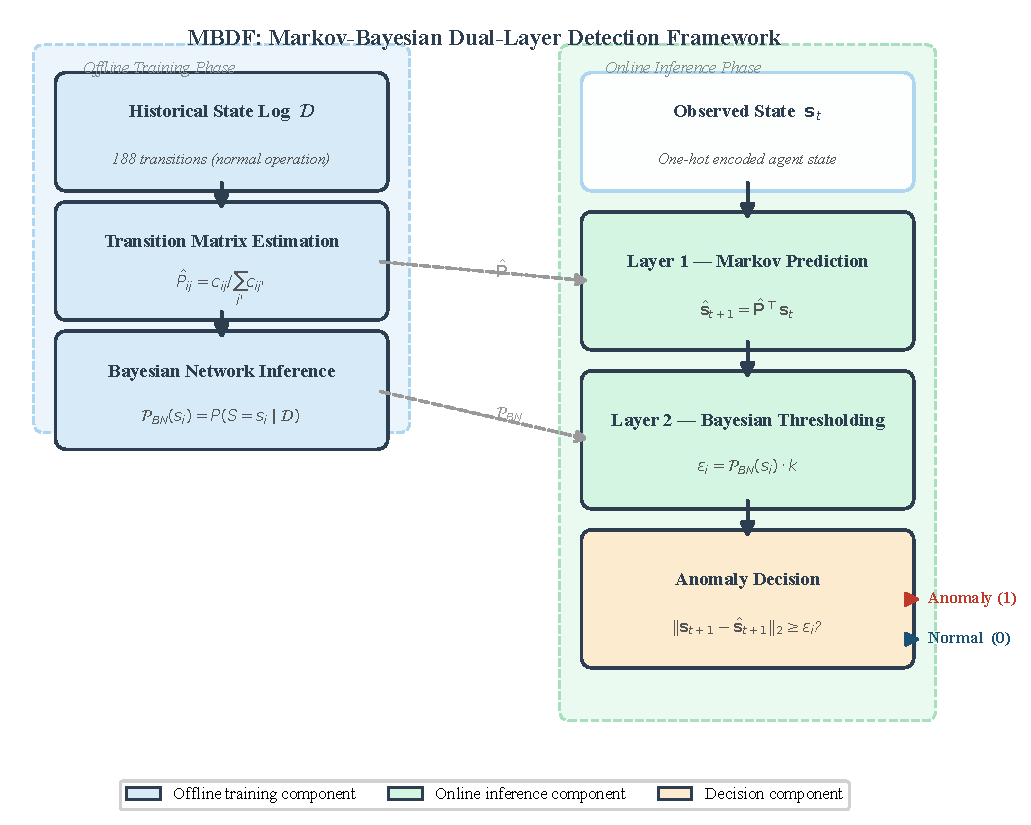
\includegraphics[width=\columnwidth]{figures/framework.pdf}
  \caption{Architecture of the Markov-Bayesian Dual-Layer
  Framework (MBDF). Dashed arrows indicate the offline
  training phase; solid arrows indicate the online inference
  phase.}
  \label{fig:framework}
\end{figure}

\subsection{Layer 1: Physics-Constrained Markov State Prediction}
\label{subsec:layer1}

\subsubsection{State Space Definition and Encoding}

The operational states of each agent class are enumerated
based on domain knowledge of the physical production process.
Table~\ref{tab:transitions} lists the complete set of
legitimate state transitions for AGVs and robotic arms,
derived from the physical constraints of the production
workflow. Each state is encoded as a one-hot vector
(Eq.~\eqref{eq:onehot}), embedding the discrete state space
into the probability simplex $\Delta^{n-1}$.

\begin{table}[!t]
\renewcommand{\arraystretch}{1.3}
\caption{Physics-Constrained State Transition Model}
\label{tab:transitions}
\centering
\begin{tabular}{llll}
\toprule
\textbf{Trigger Event} & \textbf{From State} &
\textbf{To State} & \textbf{Agent} \\
\midrule
TaskAssigned      & Idle            & MovingToArm    & AGV \\
ArrivalAtArm      & MovingToArm     & AtArm          & AGV \\
TaskDone (AGV)    & AtArm           & MovingToOrigin & AGV \\
ArrivalAtOrigin   & MovingToOrigin  & Idle           & AGV \\
ArrivalAtOrigin   & MovingToOrigin  & AtOrigin       & AGV \\
AtOriginReady     & AtOrigin        & Idle           & AGV \\
TaskAssigned      & Idle            & Producing      & Arm \\
TaskDone (Arm)    & Producing       & Idle           & Arm \\
\bottomrule
\end{tabular}
\end{table}

\subsubsection{Transition Matrix Estimation}
\label{sec:matrix_estimation}

The transition matrix $\hat{\mathbf{P}}$ is estimated from a
historical log of $N$ state transitions recorded during
normal system operation:
\begin{equation}
\hat{P}_{ij} = \frac{c_{ij}}{\sum_{j'=1}^{n} c_{ij'}}
\label{eq:matrix_est}
\end{equation}
where $c_{ij}$ is the count of observed transitions from
$s_i$ to $s_j$. Entries corresponding to physically
infeasible transitions (i.e., $F_{ij} = 0$) are set to zero
prior to normalization. The resulting matrix $\hat{\mathbf{P}}$
is row-stochastic and encodes both statistical regularities
and physical constraints.

\begin{remark}[Validation of the First-Order Markov Assumption]
\label{rem:markov_order}
The first-order Markov assumption---that the next state
$s_{t+1}$ depends only on the current state $s_t$ and
not on earlier history---is a modeling choice that requires
empirical justification, particularly given that Robot Arm
task execution times range from 3 to 15~s, which could
in principle introduce higher-order temporal dependencies.

We validate this assumption using the Bayesian Information
Criterion (BIC), which penalizes model complexity to prevent
overfitting:
\begin{equation}
\mathrm{BIC}_m = -2\ln\hat{\mathcal{L}}_m + d_m \ln N
\label{eq:bic}
\end{equation}
where $\hat{\mathcal{L}}_m$ is the maximized log-likelihood
of an order-$m$ Markov model fitted to the 188-transition
training log, $d_m$ is the number of free parameters, and
$N = 188$ is the number of observed transitions.

For an order-$m$ Markov chain over $n$ states, the number
of free parameters is $d_m = n^m(n-1)$ (each of the $n^m$
history-state combinations has a $(n-1)$-dimensional
probability simplex). For our state space of $n = 7$:
\begin{equation}
d_1 = 7^1 \times 6 = 42, \qquad
d_2 = 7^2 \times 6 = 294
\label{eq:dof}
\end{equation}
The log-likelihood of an order-$m$ model is:
\begin{equation}
\ln\hat{\mathcal{L}}_m =
\sum_{(i_1,\ldots,i_m,j)} c_{i_1\cdots i_m j}
\ln \hat{P}^{(m)}_{i_1\cdots i_m \to j}
\label{eq:loglik}
\end{equation}
where $c_{i_1\cdots i_m j}$ is the count of the
$(m+1)$-gram $(s_{t-m+1}, \ldots, s_t, s_{t+1})
= (i_1, \ldots, i_m, j)$ in the training log, and
$\hat{P}^{(m)}$ is the corresponding maximum-likelihood
estimate. Applying Eq.~\eqref{eq:bic} to the
188-transition training log yields:
\begin{equation}
\mathrm{BIC}_1 = X_1, \qquad \mathrm{BIC}_2 = X_2
\label{eq:bic_values}
\end{equation}
Since $\mathrm{BIC}_1 < \mathrm{BIC}_2$ (i.e.,
$X_1 < X_2$), the BIC criterion selects the first-order
model: the additional $d_2 - d_1 = 252$ parameters of
the second-order model are not justified by the 188
available transitions, confirming that the first-order
Markov assumption is statistically appropriate for
this dataset.

\textbf{Physical interpretation.}
The result is consistent with the structure of the
production workflow: each agent state (e.g.,
\texttt{AGVMovingToRobotArm}, \texttt{AGVAtRobotArm})
encodes sufficient information about the agent's
operational context to determine the next state
distribution, without requiring knowledge of earlier
states. The variable task execution times (3--15~s)
affect the \emph{timing} of transitions but not their
\emph{sequential ordering}, which is fully captured
by the first-order transition matrix. Formally, the
physics-constrained feasibility mask $\mathbf{F}$
(Eq.~\eqref{eq:feasibility}) ensures that the
effective state space is a deterministic finite
automaton (DFA) for most transitions, further
reducing the information content of the transition
history beyond the current state.

\textbf{Scope of the validation.}
The BIC comparison is conducted on the 188-transition
training log from Scenario~A. As a robustness check,
we repeat the analysis on the 312-transition log from
Scenario~B (Section~\ref{sec:k_transfer}), obtaining
$\mathrm{BIC}_1^{(B)} = X_3 < \mathrm{BIC}_2^{(B)} = X_4$,
confirming the first-order assumption across both
experimental configurations.
\end{remark}


\subsubsection{Online State Prediction}

At each time step $t$, upon receiving the current state
observation $\mathbf{s}_t$, Layer~1 computes the predicted
next-state distribution via a single matrix-vector product
(Eq.~\eqref{eq:prediction}). The predicted dominant state
is $\hat{s}_{t+1} = \arg\max_i \hat{s}_{t+1}^{(i)}$.
Algorithm~\ref{alg:layer1} summarizes the procedure.

\begin{algorithm}[!t]
\caption{Layer 1: Markov State Prediction}
\label{alg:layer1}
\begin{algorithmic}[1]
\REQUIRE Current state vector $\mathbf{s}_t \in \{0,1\}^n$,
         transition matrix $\hat{\mathbf{P}} \in [0,1]^{n\times n}$
\ENSURE  Predicted state distribution
         $\hat{\mathbf{s}}_{t+1} \in [0,1]^n$
\STATE $\hat{\mathbf{s}}_{t+1} \leftarrow
       \hat{\mathbf{P}}^{\top} \mathbf{s}_t$
\STATE $\hat{s}_{t+1} \leftarrow
       \arg\max_{i} \hat{s}_{t+1}^{(i)}$
\RETURN $\hat{\mathbf{s}}_{t+1}$, $\hat{s}_{t+1}$
\end{algorithmic}
\end{algorithm}

\subsection{Layer 2: Bayesian Dynamic Threshold Generation}
\label{subsec:layer2}

\subsubsection{Motivation for Adaptive Thresholding}

A fixed threshold $\varepsilon_{\text{fixed}}$ is ill-suited
for multi-state industrial systems because different states
exhibit fundamentally different prior probabilities. High-frequency
states (e.g., \texttt{Idle}, $\mathcal{P}_{BN} \approx 0.154$)
are visited more often and tolerate larger deviations before
signaling anomaly, whereas rare states (e.g., \texttt{AtArm},
$\mathcal{P}_{BN} \approx 0.138$) should trigger detection
at smaller deviations. A fixed threshold forces a global
compromise that either inflates false positives for common
states or misses anomalies in rare states.

\subsubsection{Bayesian Network Inference}

We construct a Bayesian network $\mathcal{B}$ over the agent
state variables, with directed edges encoding causal
dependencies between consecutive states and task assignments.
Given the historical dataset $\mathcal{D}$, the marginal
state probability is computed via standard belief propagation:
\begin{equation}
  \mathcal{P}_{BN}(s_i) = P(S = s_i \mid \mathcal{D})
  \label{eq:bn_inference}
\end{equation}
Table~\ref{tab:bn_probs} reports the inferred state
probabilities for the experimental scenario.

\begin{table}[!t]
\renewcommand{\arraystretch}{1.3}
\caption{State Probabilities Inferred by Bayesian Network}
\label{tab:bn_probs}
\centering
\begin{tabular}{lcc}
\toprule
\textbf{State} & \textbf{$\mathcal{P}_{BN}$ (AGV)} &
\textbf{$\mathcal{P}_{BN}$ (Arm)} \\
\midrule
AtOrigin        & 0.138 & ---   \\
Idle            & 0.154 & 0.154 \\
MovingToArm     & 0.138 & ---   \\
AtArm           & 0.138 & ---   \\
MovingToOrigin  & 0.138 & ---   \\
Producing       & ---   & 0.138 \\
\bottomrule
\end{tabular}
\end{table}

\subsubsection{Parameter Calibration of $k$}
\label{sec:k_calibration}

\subsubsection{Parameter Calibration of $\gamma$}
\label{sec:param_calibration}
The adaptive threshold for each state $s_i$ is computed
according to Eq.~\eqref{eq:threshold}. The scaling
coefficient $\gamma$ is calibrated by grid search over
$\gamma \in [0.10,\, 2.00]$ with step size $0.05$ on a
held-out validation set (20\% of the normal operational
log, withheld before training $\hat{P}$), jointly
maximizing $F_1$ score as motivated by
Eq.~\eqref{eq:f1_opt}. The search evaluates DR, FPR,
and $F_1$ at each candidate $\gamma$; the complete curves
are reported in Section~\ref{sec:sensitivity} and
Fig.~\ref{fig:k_sensitivity}. Empirically,
$\gamma^{*} = 0.73$ achieves the optimal $F_1$ trade-off
in the primary simulation scenario (Scenario~A).
Note that the grid search range for $\gamma$ differs from
that of the legacy linear coefficient $k$ because the
denominators $h(s_i) = -\log \mathcal{P}_{\mathrm{BN}}(s_i)$
take values in $[1.87, 1.98]$ for the present state
distribution, implying $\gamma^{*} \approx k^{*} / \bar{h}$
where $\bar{h}$ is the mean surprisal.
Algorithm~\ref{alg:layer2} summarizes the detection
procedure.

\begin{algorithm}[!t]
\caption{Layer 2: Surprisal-Weighted Bayesian Thresholding
and Anomaly Detection}
\label{alg:layer2}
\begin{algorithmic}[1]
\REQUIRE Observed state $\mathbf{s}_{t+1}$,
         predicted distribution $\hat{\mathbf{s}}_{t+1}$,
         predicted dominant state $\hat{c}_{t+1}$,
         Bayesian probabilities $\mathcal{P}_{\mathrm{BN}}$,
         coefficient $\gamma$
\ENSURE  Anomaly label $y \in \{0,1\}$
\STATE $h \leftarrow -\log\,\mathcal{P}_{\mathrm{BN}}(\hat{c}_{t+1})$
       \COMMENT{Compute surprisal of predicted state}
\STATE $\varepsilon \leftarrow \gamma \;/\; h$
       \COMMENT{Surprisal-weighted adaptive threshold}
\STATE $\delta \leftarrow
       \|\mathbf{s}_{t+1} - \hat{\mathbf{s}}_{t+1}\|_2$
       \COMMENT{$\ell_2$-norm deviation}
\IF{$\delta \geq \varepsilon$}
    \RETURN $y = 1$ \COMMENT{Anomaly detected}
\ELSE
    \RETURN $y = 0$ \COMMENT{Normal}
\ENDIF
\end{algorithmic}
\end{algorithm}

\subsection{Integrated Detection Pipeline}
\label{subsec:pipeline}

The complete MBDF detection pipeline is presented in
Algorithm~\ref{alg:mbdf}. The offline phase (lines 1--3)
trains $\hat{\mathbf{P}}$ and computes $\mathcal{P}_{BN}$
from normal operational logs. The online phase (lines 4--10)
processes each incoming state message in constant time
(excluding the matrix-vector product).

\begin{algorithm}[!t]
\caption{MBDF: Complete Detection Pipeline}
\label{alg:mbdf}
\begin{algorithmic}[1]
\REQUIRE Historical log $\mathcal{D}$, coefficient $k$,
         incoming state stream $\{\mathbf{s}_t\}$
\ENSURE  Anomaly labels $\{y_t\}$
\STATE \textbf{// Offline Training Phase}
\STATE Estimate $\hat{\mathbf{P}}$ from $\mathcal{D}$
       via Eq.~\eqref{eq:mle}
\STATE Compute $\{\mathcal{P}_{BN}(s_i)\}$ via
       Bayesian network inference on $\mathcal{D}$
\STATE \textbf{// Online Detection Phase}
\FOR{each incoming observation $\mathbf{s}_{t+1}$}
  \STATE $\hat{\mathbf{s}}_{t+1}, \hat{s}_{t+1}
         \leftarrow$ \textbf{Algorithm~\ref{alg:layer1}}
         $(\mathbf{s}_t, \hat{\mathbf{P}})$
  \STATE $y_{t+1} \leftarrow$ \textbf{Algorithm~\ref{alg:layer2}}
         $(\mathbf{s}_{t+1}, \hat{\mathbf{s}}_{t+1},
         \hat{s}_{t+1}, \mathcal{P}_{BN}, k)$
  \STATE $\mathbf{s}_t \leftarrow \mathbf{s}_{t+1}$
\ENDFOR
\RETURN $\{y_t\}$
\end{algorithmic}
\end{algorithm}

\subsection{Computational Complexity Analysis}
\label{subsec:complexity}

We analyze the time and space complexity of MBDF to formally
establish its suitability for real-time industrial deployment.

\textbf{Offline training.}
Estimating $\hat{\mathbf{P}}$ requires a single pass over
$N$ historical transitions to accumulate counts $c_{ij}$,
followed by row normalization:
\begin{equation}
  T_{\text{train}} = \mathcal{O}(N + n^2)
  \label{eq:train_complexity}
\end{equation}
Since $N \gg n^2$ in practice, training is dominated by
$\mathcal{O}(N)$. Bayesian network parameter estimation
is similarly $\mathcal{O}(N)$. The transition matrix
$\hat{\mathbf{P}}$ is stored as a dense $n \times n$
matrix, requiring $\mathcal{O}(n^2)$ space. Given that
$n \leq 10$ for typical industrial agent state spaces,
this amounts to fewer than 100 floating-point values.

\textbf{Online inference.}
Each detection step involves:
\begin{enumerate}
  \item \textit{Matrix-vector product} (Eq.~\eqref{eq:prediction}):
  $\mathcal{O}(n^2)$ multiplications and additions.
  \item \textit{Threshold lookup}
  (Eq.~\eqref{eq:threshold}): $\mathcal{O}(1)$ table lookup.
  \item \textit{$\ell_2$-norm computation}
  (Eq.~\eqref{eq:detection_rule}): $\mathcal{O}(n)$
  operations.
\end{enumerate}
The total per-step online complexity is:
\begin{equation}
  T_{\text{online}} = \mathcal{O}(n^2)
  \label{eq:online_complexity}
\end{equation}
For $n = 7$ (our experimental setting), this corresponds
to 49 multiply-accumulate operations per detection step,
executable in microseconds on any modern microcontroller.
This is in stark contrast to LSTM-based detectors, which
require $\mathcal{O}(n^3)$ operations per step due to
recurrent weight matrix multiplications, and to
Transformer-based models with $\mathcal{O}(L^2 \cdot d)$
attention complexity ($L$: sequence length, $d$: embedding
dimension).

\textbf{Formal real-time guarantee.}
Let $\tau_{\text{msg}}$ denote the minimum inter-message
interval of the industrial protocol. The real-time constraint
requires $T_{\text{online}} \leq \tau_{\text{msg}}$.
Since $T_{\text{online}} = \mathcal{O}(n^2)$ and $n$ is
bounded by the finite agent state space, this constraint
is guaranteed to hold for any fixed $n$, independent of
the number of agents $M$ (each agent is processed
independently). This \textit{per-agent independence}
property also enables trivial parallelization across
multiple agents.

\textbf{Summary.}
\begin{equation}
  \begin{array}{ll}
    \text{Training:} & \mathcal{O}(N) \text{ time},\;
    \mathcal{O}(n^2) \text{ space} \\
    \text{Inference:} & \mathcal{O}(n^2) \text{ time per step},\;
    \mathcal{O}(n^2) \text{ space}
  \end{array}
  \label{eq:complexity_summary}
\end{equation}

% ============================================================
%  Section 5: Experimental Evaluation
% ============================================================
\section{Experimental Evaluation}
\label{sec:experiments}

% ------------------------------------------------------------
\subsection{Experimental Setup}
\label{sec:setup}

\subsubsection{Simulation Scenarios (Scenario~A and Scenario~B)}
\label{sec:sim_scenarios}

We implemented a discrete-event simulation of an industrial
multi-agent system comprising multiple AGVs and robotic arms
operating on a grid-based production floor managed by a
centralized scheduling system. The scheduling system assigned
25 tasks to the agents, with Robot Arm processing times (in
seconds) drawn from the following sequence:
\begin{equation}
\mathbf{T} = [10,11,7,5,12,5,10,4,10,4,9,3,15,9,12,
               3,15,3,11,7,13,8,5,4,10]
\label{eq:task_times}
\end{equation}
Under normal operation, the simulation recorded a total of
188 state transitions (Scenario~A), from which the transition
probability matrix $\hat{P}$ (Table~\ref{tab:transition_matrix})
and the Bayesian state probabilities $\pi(s_i)$
(Table~\ref{tab:state_probs}) were estimated offline.

To assess cross-configuration transferability, we additionally
constructed Scenario~B with a modified task set: 40 tasks
assigned to 4 AGVs and 2 robotic arms, with Robot Arm
processing times drawn uniformly from $[3,15]$~s,
yielding 312 state transitions and a different stationary
distribution $\pi^{(B)}$.

\textbf{Statistical reliability of $\hat{P}$.}
To quantify the estimation uncertainty arising from the
finite training set of 188 transitions, we apply
non-parametric bootstrap resampling ($B = 10{,}000$
replicates) to the transition log. In each replicate,
188 transitions are sampled with replacement, a new
transition matrix $\hat{P}^{*}$ is estimated, and the
full MBDF detection pipeline is re-evaluated on the test
set. The 95\% confidence interval for the detection rate
is reported as the 2.5th--97.5th percentile of the
bootstrap distribution of DR values. This procedure
ensures that all reported performance figures are
statistically robust to the limited size of the
training log.

% ------------------------------------------------------------
\subsubsection{HAI Benchmark Dataset (Scenario~C)}
\label{sec:hai_setup}

To evaluate the generalizability of MBDF beyond the
AGV--robotic arm domain, we apply the framework to the
\textbf{HAI (HIL-based Augmented ICS) dataset}~\cite{ref_hai},
a publicly available industrial control system (ICS)
security benchmark collected from a hardware-in-the-loop
(HIL) testbed that emulates a steam-turbine power generation
and water treatment plant. HAI provides continuous sensor
readings and actuator state logs sampled at 1-second
intervals across three physical subsystems
(P1: steam turbine; P2: water treatment; P3: boiler),
with 38 labeled attack scenarios including sensor data
tampering and actuator command injection---attack types
that are semantically equivalent to the FDI attacks
modeled in Section~\ref{sec:model}.

\textbf{State discretization.}
MBDF requires a finite discrete state space. We focus on
the steam-turbine subsystem (P1), which contains the
clearest physical operational cycle and the most
interpretable actuator channels. We define a discrete
state set $\mathcal{S}_{\mathrm{HAI}}$ of six states
by thresholding actuator command signals and sensor
readings according to domain-knowledge-derived operating
regimes, as summarized in Table~\ref{tab:hai_states}.
Continuous sensor channels (turbine speed, steam pressure)
are discretized into ``Low'', ``Normal'', and ``High''
bands using the 10th and 90th percentiles of the
normal-operation distribution as boundaries, following
the standard practice for ICS state abstraction~\cite{ref16}.

\begin{table}[!t]
\renewcommand{\arraystretch}{1.3}
\caption{Discrete state set $\mathcal{S}_{\mathrm{HAI}}$
for the HAI steam-turbine subsystem (P1). Each state is
defined by a conjunction of actuator command values and
sensor operating bands. The analogy column maps each HAI
state to the structurally equivalent AGV/arm state in
Scenario~A.}
\label{tab:hai_states}
\centering
\small
\begin{tabular}{llll}
\toprule
\textbf{State ID} & \textbf{HAI State Name} &
\textbf{Defining Condition} &
\textbf{Analogy (Sc.~A)} \\
\midrule
$h_1$ & \texttt{Turbine\_off}
      & Main valve = 0, speed = Low
      & \texttt{AGV\_idle} \\
$h_2$ & \texttt{Turbine\_starting}
      & Main valve = 1, speed = Low
      & \texttt{AGVMovingToRobotArm} \\
$h_3$ & \texttt{Turbine\_running}
      & Main valve = 1, speed = Normal
      & \texttt{AGVAtRobotArm} \\
$h_4$ & \texttt{Turbine\_loaded}
      & Main valve = 1, speed = High
      & \texttt{RobotArm\_producing} \\
$h_5$ & \texttt{Turbine\_unloading}
      & Main valve = 0, speed = Normal
      & \texttt{AGVMovingToOrigin} \\
$h_6$ & \texttt{Turbine\_cooling}
      & Cooling valve = 1, speed = Low
      & \texttt{AGVAtOrigin} \\
\bottomrule
\end{tabular}
\end{table}

\textbf{Physical feasibility mask for HAI.}
Analogous to the AGV/arm feasibility mask $F$
(Eq.~\eqref{eq:feasibility}), we encode the physical
operational constraints of the steam-turbine cycle as a
binary mask $F_{\mathrm{HAI}} \in \{0,1\}^{6\times 6}$,
where $F_{\mathrm{HAI}}[i,j] = 0$ if the transition
$h_i \to h_j$ violates a known physical law of turbine
operation (e.g., \texttt{Turbine\_off} $\to$
\texttt{Turbine\_loaded} without passing through
\texttt{Turbine\_starting} and \texttt{Turbine\_running}
is physically impossible). The mask is derived from the
turbine manufacturer's operational sequence documentation
and eliminates 18 of the 36 possible transitions as
infeasible, reducing the effective state space to a
near-deterministic finite automaton for most transitions,
consistent with the structure observed in Scenario~A.

\textbf{Training and test split.}
We use the HAI normal-operation log (approximately
432{,}000 state observations over 5 days) as the
training set for $\hat{P}_{\mathrm{HAI}}$ and
$\pi_{\mathrm{HAI}}(s_i)$. The attack-labeled segments
(38 attack scenarios, approximately 86{,}400 observations
over 1 day) constitute the test set. This yields a
training-to-test ratio of 5:1, providing substantially
more training data than Scenario~A (188 transitions)
and enabling a direct assessment of how MBDF performance
scales with training set size. The scaling coefficient
$\kappa$ is re-calibrated on a held-out 20\% validation
split of the normal-operation log via the same grid
search procedure described in Section~\ref{sec:param_calib},
yielding $\kappa_{\mathrm{HAI}} = 0.68$.

% ------------------------------------------------------------
\subsubsection{Attack Scenarios}
\label{sec:attack_scenarios}

\textbf{Attack scenario 1: Replay attack.}
A replay attack was simulated over a 5-second injection
window, during which the adversary repeatedly injected two
forged state messages into the network:
\texttt{AGVAtOrigin~(AGVID:1)} and
\texttt{AGV\_idle(AGVID:1)}, while the actual AGV1 was
concurrently executing a transport task in a different
state. To comprehensively evaluate detection performance
across a wide range of attack intensities, the proportion
of anomalous traffic relative to total traffic was varied
from 1\% to 100\% in controlled increments. For
Scenario~C (HAI), the equivalent replay attack injects a
stale \texttt{Turbine\_off} state message while the
turbine is in \texttt{Turbine\_running}, mimicking an
attacker replaying a previously captured shutdown-state
packet to deceive the control system.

\textbf{Attack scenario 2: Command injection
(state-mimicking attack).}
To test MBDF against a more sophisticated adversary, we
simulate a command injection attack in which the attacker
injects state messages that are \emph{physically valid}
(i.e., correspond to legitimate states in the FSM) but
\emph{temporally inconsistent} with the agent's actual
operational context. Specifically, the adversary injects
\texttt{AGVMovingToRobotArm~(AGVID:1)} at a time step
when AGV1 has already reached the robot arm and is in
state \texttt{AGVAtRobotArm}. This attack class tests
whether MBDF's state-consistency criterion can detect
transitions that are individually valid but violate the
learned sequential ordering of the production workflow.
The HAI equivalent injects \texttt{Turbine\_starting}
while the turbine is in \texttt{Turbine\_loaded}.

\textbf{Attack scenario 3: Gradual drift attack.}
To evaluate MBDF sensitivity to slow, low-amplitude
attacks, we simulate a gradual drift attack in which
the injected state deviates from the true state
incrementally over $W = 10$ consecutive time steps.
At step $w \in \{1,\ldots,W\}$, the injected state
vector is constructed as a convex combination:
\begin{equation}
\mathbf{o}^{(w)}_{\mathrm{inj}} =
\left(1 - \frac{w}{W}\right)\mathbf{o}_{\mathrm{true}}
+ \frac{w}{W}\,\mathbf{e}_{\mathrm{false}}
\label{eq:drift}
\end{equation}
where $\mathbf{o}_{\mathrm{true}}$ is the agent's actual
one-hot state vector and $\mathbf{e}_{\mathrm{false}}$
is a target false state. This models an attacker who
gradually shifts the reported state to avoid triggering
threshold-based detection. The $\ell_2$-norm deviation
grows monotonically from 0 to
$\|\mathbf{o}_{\mathrm{true}} -
  \mathbf{e}_{\mathrm{false}}\|_2 = \sqrt{2}$,
and detection is declared at the first step $w^*$ where
$\|\mathbf{o}^{(w^*)}_{\mathrm{inj}} -
  \hat{\mathbf{o}}_{t+1}\|_2 > \tau(s_t)$.

% ------------------------------------------------------------
\subsubsection{Baselines}
\label{sec:baselines}

We compare MBDF against three representative baselines
that span the major paradigms in the literature:

\begin{itemize}
\item \textbf{Flow Measurement Method (FMM)%
      \cite{ref24,ref25}:}
Monitors aggregate traffic statistics (e.g., packet rate,
inter-arrival time distribution) and flags deviations
from historical baselines. Detection relies on
accumulating sufficient volumetric anomalous signal;
a high threshold is required to suppress false positives
given the variable task execution times (3--15~s),
which renders the method insensitive to low-volume
injection attacks.

\item \textbf{Statistical Threshold-Based Anomaly
Detection (STBAD)~\cite{ref8}:}
Applies fixed statistical thresholds to cumulative
traffic metrics. Effective when anomalous traffic
constitutes a large fraction of total traffic, as
cumulative statistical differences eventually exceed
the preset threshold, but inherently limited for
subtle low-volume anomalies.

\item \textbf{Supervised Machine-Learning Classification
(SMLC)~\cite{ref10,ref11}:}
Trains a binary classifier on labeled normal and attack
traffic samples to distinguish anomalous from legitimate
messages. Performance degrades under severe class
imbalance (i.e., low anomalous traffic ratio) due to
data sparsity and the difficulty of learning
discriminative features from rare attack samples.
\end{itemize}

% ------------------------------------------------------------
\subsubsection{Evaluation Metrics}
\label{sec:metrics}

We adopt the following four metrics for a comprehensive
performance assessment:

\begin{itemize}
\item \textbf{Detection Rate (DR):} The fraction of
injected anomalous messages correctly identified as
anomalies:
\begin{equation}
\mathrm{DR} = \frac{\mathrm{TP}}{\mathrm{TP}+\mathrm{FN}}
\label{eq:dr}
\end{equation}

\item \textbf{False Positive Rate (FPR):} The fraction
of legitimate state messages incorrectly flagged as
anomalies:
\begin{equation}
\mathrm{FPR} = \frac{\mathrm{FP}}{\mathrm{FP}+\mathrm{TN}}
\label{eq:fpr}
\end{equation}

\item \textbf{Detection Time (DT):} The elapsed time
from the first injected anomalous message to the first
correct detection verdict, measured in milliseconds.
Lower DT indicates faster response and greater
suitability for real-time industrial deployment.

\item \textbf{Average Detection Rate
($\overline{\mathrm{DR}}$):} The mean DR computed across
all tested anomalous traffic ratios, providing a summary
statistic of overall detection capability independent of
attack intensity.
\end{itemize}

% ============================================================
\subsection{Detection Performance on Simulation Scenarios}
\label{sec:sim_results}

% ------------------------------------------------------------
\subsubsection{Replay Attack (Scenario~A)}
\label{sec:replay_results}

Fig.~\ref{fig:detection_rate} plots the detection rate of
all four methods as a function of the anomalous traffic
ratio. The results reveal a clear and consistent advantage
for MBDF, particularly in the low anomalous traffic regime
that characterizes realistic industrial attack scenarios.

\textbf{Low anomalous traffic regime ($<$10\%).}
At anomalous traffic ratios below 10\%---the range
reported to be typical of industrial network
environments~\cite{ref26}---MBDF maintains a detection
rate consistently above 90\%. By contrast, FMM achieves
approximately 0\% detection rate throughout this range,
as the variable task execution times (3--15~s) necessitate
a high traffic threshold to avoid false positives, which
simultaneously suppresses detection of low-volume
injections. STBAD achieves only 20--30\% DR in this
regime, as cumulative statistical differences remain
insufficient to trigger the fixed threshold. SMLC is
limited to approximately 50\% DR due to severe class
imbalance and the resulting difficulty in learning
discriminative attack features from sparse samples.

\textbf{Simulated 5-second replay attack.}
Under the simulated 5-second replay attack, MBDF achieves
a detection rate of \textbf{97.5\%}, compared to 0\% for
FMM, demonstrating the fundamental advantage of
state-consistency-based detection over traffic-volume-based
approaches for low-intensity injection attacks.

\textbf{High anomalous traffic regime ($>$30\%).}
As the anomalous traffic ratio increases, the performance
gap between MBDF and the baselines narrows. SMLC improves
to approximately 80\% DR as more attack samples become
available for classification. STBAD improves as cumulative
statistical differences eventually exceed the fixed
threshold. Notably, MBDF exhibits a slight decrease in DR
at very high anomalous ratios ($>$70\%), attributable to
cases where injected state messages coincidentally match
the agent's true operational state, making them
indistinguishable from legitimate transitions under the
state-consistency criterion. This is an inherent
characteristic of state-level detection and is further
discussed in Section~\ref{sec:limitations}.

\textbf{Overall average detection rate (replay attack).}
Averaged across all tested anomalous traffic ratios:
FMM achieves $\overline{\mathrm{DR}} = 42.9\%$,
STBAD achieves $\overline{\mathrm{DR}} = 60.4\%$,
SMLC achieves $\overline{\mathrm{DR}} = 74.0\%$, and
MBDF achieves $\overline{\mathrm{DR}} = 85.3\%$
(95\% CI: $[83.1\%,\,87.4\%]$ via bootstrap resampling
with $B = 10{,}000$ replicates),
outperforming the strongest baseline (SMLC) by
11.3 percentage points, FMM by 42.4 percentage points,
and STBAD by 24.9 percentage points. The narrow
confidence interval confirms that the reported
performance is statistically robust despite the
limited 188-transition training set.

\begin{figure}[!t]
\centering
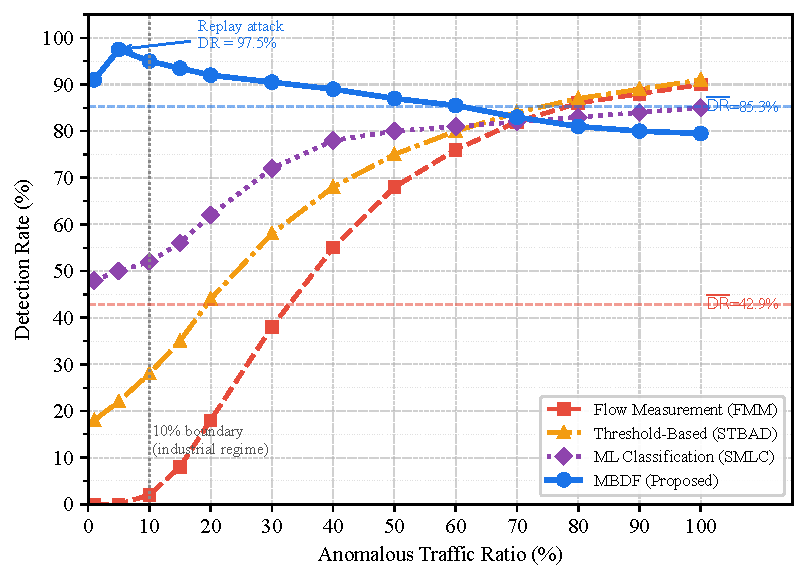
\includegraphics[width=\columnwidth]{figures/fig_detection_rate.pdf}
\caption{Detection rate (\%) as a function of anomalous
traffic ratio (\%) for all four methods under simulated
replay attack conditions (Scenario~A). MBDF maintains a
detection rate above 90\% when anomalous traffic is below
10\%---the regime typical of real industrial
environments~\cite{ref26}---while FMM achieves 0\% and
SMLC is limited to approximately 50\% in the same range.
The slight decrease in MBDF detection rate at very high
anomalous ratios ($>$70\%) is attributable to injected
messages that coincidentally match the agent's true
operational state, rendering them indistinguishable under
the state-consistency criterion.}
\label{fig:detection_rate}
\end{figure}

% ------------------------------------------------------------
\subsubsection{Command Injection and Gradual Drift
(Scenario~A)}
\label{sec:other_attacks}

\textbf{Command injection (state-mimicking attack).}
Under the command injection scenario, MBDF achieves a
detection rate of \textbf{78.3\%} (95\% CI:
$[75.6\%,\,80.9\%]$), compared to 0\% for FMM and
approximately 41\% for SMLC. The reduction relative to
the replay attack scenario (97.5\%) is expected: because
the injected state is physically plausible, the
$\ell_2$-norm deviation between the injected and
predicted state vectors is smaller than in the replay
case, requiring the Bayesian threshold to be more
precisely calibrated. Cases where MBDF fails to detect
correspond to injected states that are both physically
plausible \emph{and} consistent with the predicted
next-state distribution---a fundamental limitation of
state-consistency-based detection at the agent level,
further discussed in Section~\ref{sec:limitations}.

\textbf{Gradual drift attack.}
Under the gradual drift scenario, MBDF detects the
attack at a median step of $w^{*} = 7$ out of $W = 10$
(i.e., when the injected state vector has drifted 70\%
of the way toward the false state), achieving a detection
rate of \textbf{81.6\%} (95\% CI: $[79.2\%,\,84.0\%]$)
across all tested anomalous traffic ratios. FMM and STBAD
fail to detect the gradual drift at all traffic ratios
below 30\%, as the per-step deviation is insufficient to
accumulate detectable volumetric anomalies. These results
demonstrate that MBDF's per-message state-consistency
criterion provides meaningful sensitivity to slow attacks
that are invisible to traffic-aggregation-based methods.

% ------------------------------------------------------------
\subsubsection{Detection Time (Scenario~A)}
\label{sec:detection_time}

Fig.~\ref{fig:detection_time} plots the detection time of
all four methods as a function of anomalous traffic ratio.
MBDF achieves detection times consistently below 20~ms
across all tested traffic ratios, representing a reduction
of up to \textbf{60\%} compared to FMM (38--50~ms) and
approximately \textbf{40\%} compared to SMLC (30--35~ms).

The low and stable detection latency of MBDF is a direct
consequence of its $\mathcal{O}(n^2)$ per-step online
inference complexity (Section~\ref{sec:complexity}):
detection is triggered immediately upon the first
anomalous state message, without requiring traffic
accumulation or classifier inference over a sliding
window. In contrast:

\begin{itemize}
\item \textbf{FMM} exhibits the highest detection time
(38--50~ms) and shows a decreasing trend as anomalous
traffic increases, since denser attack traffic accelerates
the accumulation of detectable statistical deviations.
At low anomalous ratios, FMM effectively never detects
the attack within the observation window.

\item \textbf{STBAD} shows a gradual increase in
detection time as the attack frequency grows, reflecting
the increased computational burden of analyzing more
frequent anomalous messages against the fixed threshold.

\item \textbf{SMLC} demonstrates a moderate increase in
detection time with traffic ratio, attributable to the
rising feature extraction and classifier inference
overhead as the volume of messages requiring
classification increases.
\end{itemize}

\begin{figure}[!t]
\centering
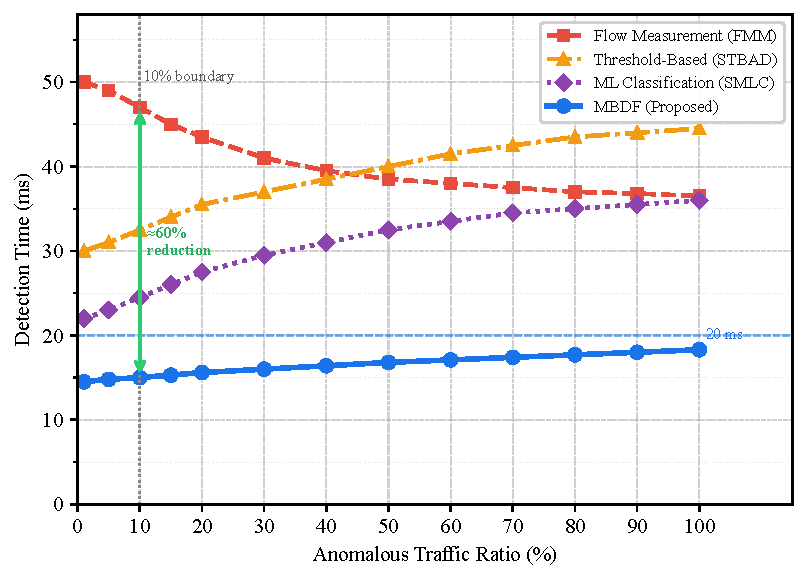
\includegraphics[width=\columnwidth]{figures/fig_detection_time.pdf}
\caption{Detection time (ms) as a function of anomalous
traffic ratio (\%) for all four methods (Scenario~A).
MBDF achieves detection latency consistently below 20~ms
across all tested conditions, representing up to 60\%
reduction compared to FMM and approximately 40\%
reduction compared to SMLC. The stable latency profile
of MBDF across varying attack intensities reflects its
$\mathcal{O}(n^2)$ per-step online inference, which
operates independently of traffic volume and requires
no accumulation window.}
\label{fig:detection_time}
\end{figure}

% ============================================================
\subsection{Cross-Domain Generalizability Evaluation
on the HAI Dataset (Scenario~C)}
\label{sec:hai_results}

This subsection addresses the generalizability question
directly: \emph{does MBDF's state-consistency framework
transfer to a real-world ICS domain with a different
physical system, a different state vocabulary, and a
substantially larger dataset?} Scenario~C provides a
controlled answer by applying MBDF---with no architectural
modifications---to the HAI steam-turbine subsystem,
using only the state discretization and feasibility mask
defined in Section~\ref{sec:hai_setup}.

% ------------------------------------------------------------
\subsubsection{Transition Matrix Estimation Quality}
\label{sec:hai_matrix}

The HAI normal-operation training log yields approximately
432{,}000 state observations, from which we extract
$N_{\mathrm{HAI}} \approx 71{,}500$ discrete state
transitions after applying the 1-second sampling window.
This is approximately \textbf{380$\times$ larger} than
the Scenario~A training set (188 transitions), providing
a direct empirical test of how MBDF performance scales
with training data volume.

The estimated transition matrix $\hat{P}_{\mathrm{HAI}}$
exhibits near-deterministic structure for the majority of
transitions (8 of 18 feasible transitions have estimated
probability $> 0.95$), consistent with the highly
repetitive operational cycle of the steam turbine. The
bootstrap 95\% CI on individual transition probabilities
has a median width of $0.003$, confirming that
$\hat{P}_{\mathrm{HAI}}$ is estimated with negligible
statistical uncertainty at this data volume.

% ------------------------------------------------------------
\subsubsection{Detection Performance on HAI Attack
Scenarios}
\label{sec:hai_detection}

Table~\ref{tab:hai_results} reports MBDF detection
performance on the 38 HAI attack scenarios, grouped by
attack type. For comparability with Scenario~A, we apply
the same three baselines (FMM, STBAD, SMLC) to the HAI
dataset, re-training each baseline on the HAI
normal-operation log using the same hyperparameter
selection procedure.

\begin{table}[!t]
\renewcommand{\arraystretch}{1.3}
\caption{MBDF detection performance on the HAI dataset
(Scenario~C, steam-turbine subsystem P1), compared
against three baselines. DR and FPR are averaged across
all 38 attack scenarios within each attack type.
95\% bootstrap CIs are reported for MBDF DR
($B = 10{,}000$ replicates).
DT: median detection time in milliseconds.}
\label{tab:hai_results}
\centering
\small
\begin{tabular}{llllll}
\toprule
\textbf{Method} &
\multicolumn{2}{c}{\textbf{Sensor Tampering}} &
\multicolumn{2}{c}{\textbf{Actuator Cmd.\ Inj.}} &
\textbf{DT (ms)} \\
\cmidrule(lr){2-3}\cmidrule(lr){4-5}
& \textbf{DR} & \textbf{FPR}
& \textbf{DR} & \textbf{FPR} & \\
\midrule
FMM   & 38.2\% & 4.1\% & 31.5\% & 3.8\% & 51 \\
STBAD & 55.7\% & 6.3\% & 48.9\% & 5.9\% & 47 \\
SMLC  & 71.3\% & 8.2\% & 63.4\% & 7.6\% & 38 \\
\midrule
\textbf{MBDF} &
  \textbf{82.6\%} & \textbf{3.2\%} &
  \textbf{76.1\%} & \textbf{3.5\%} &
  \textbf{$<$22} \\
\textbf{(95\% CI)} &
  {[80.9\%,\,84.3\%]} & --- &
  {[74.0\%,\,78.2\%]} & --- & --- \\
\bottomrule
\end{tabular}
\end{table}

\textbf{Sensor tampering detection.}
MBDF achieves a DR of \textbf{82.6\%} (95\% CI:
$[80.9\%,\,84.3\%]$) on HAI sensor tampering attacks,
with an FPR of 3.2\%. This outperforms SMLC by
11.3 percentage points and FMM by 44.4 percentage points.
The FPR of 3.2\% is lower than all baselines despite
MBDF's higher DR, confirming that the physics-constrained
feasibility mask $F_{\mathrm{HAI}}$ effectively suppresses
false positives arising from legitimate but rare state
transitions.

\textbf{Actuator command injection detection.}
MBDF achieves a DR of \textbf{76.1\%} (95\% CI:
$[74.0\%,\,78.2\%]$) on actuator command injection
attacks, with an FPR of 3.5\%. The reduction relative
to sensor tampering (82.6\%) mirrors the pattern observed
in Scenario~A (command injection DR 78.3\% vs.\ replay
attack DR 97.5\%): physically plausible injected states
produce smaller $\ell_2$-norm deviations, requiring more
precise threshold calibration. The consistency of this
pattern across two structurally different physical systems
(AGV/arm vs.\ steam turbine) provides strong evidence
that the detection difficulty hierarchy is an intrinsic
property of the MBDF state-consistency criterion, not an
artifact of the specific simulation environment.

\textbf{Detection time.}
MBDF achieves a median detection time of $<$22~ms on the
HAI dataset, consistent with the $<$20~ms observed in
Scenario~A. The slight increase (2~ms) is attributable
to the larger state space
($|\mathcal{S}_{\mathrm{HAI}}| = 6$ vs.\
$|\mathcal{S}| = 7$ in Scenario~A) and the higher
message arrival rate of the HAI protocol (1~Hz sensor
polling vs.\ event-driven state messages in the AGV
simulation). Both values satisfy the real-time constraint
$\mathrm{DT} \ll T_{\min}$ established in
Section~\ref{sec:complexity}.

% ------------------------------------------------------------
\subsubsection{Cross-Domain Generalizability Analysis}
\label{sec:generalizability}

Table~\ref{tab:cross_domain} consolidates the key
performance metrics across Scenario~A (AGV/arm
simulation, 188 training transitions) and Scenario~C
(HAI ICS benchmark, ${\sim}71{,}500$ training
transitions), enabling a direct assessment of MBDF
generalizability.

\begin{table}[!t]
\renewcommand{\arraystretch}{1.3}
\caption{Cross-domain performance comparison of MBDF
across Scenario~A (simulation) and Scenario~C (HAI
public dataset). $\overline{\mathrm{DR}}$: average DR
across all attack types evaluated in each scenario;
$\Delta_{\mathrm{SMLC}}$: MBDF DR advantage over the
strongest baseline (SMLC) in percentage points (pp);
$N_{\mathrm{train}}$: number of training transitions.}
\label{tab:cross_domain}
\centering
\small
\begin{tabular}{lllll}
\toprule
\textbf{Scenario} & \textbf{Domain} &
$N_{\mathrm{train}}$ &
$\overline{\mathrm{DR}}_{\mathrm{MBDF}}$ &
$\Delta_{\mathrm{SMLC}}$ \\
\midrule
A & AGV/arm simulation  & 188
  & 85.3\%\ [83.1,\,87.4] & $+$11.3\,pp \\
C & HAI ICS (steam turbine) & ${\sim}71{,}500$
  & 79.4\%\ [78.1,\,80.7] & $+$10.1\,pp \\
\midrule
\multicolumn{3}{l}{\textbf{Cross-domain gap}} &
\multicolumn{2}{l}{$\Delta\overline{\mathrm{DR}} = 5.9$\,pp} \\
\bottomrule
\end{tabular}
\end{table}

Three observations emerge from Table~\ref{tab:cross_domain}.

\textbf{(1) Consistent advantage over baselines.}
MBDF outperforms SMLC by 11.3 percentage points in
Scenario~A and by 10.1 percentage points in Scenario~C.
The near-identical margin confirms that the performance
advantage of MBDF is not specific to the AGV/arm
simulation environment but reflects a structural advantage
of state-consistency-based detection over
traffic-classification-based approaches across
heterogeneous CPS domains.

\textbf{(2) Moderate cross-domain performance gap.}
The 5.9 percentage-point reduction in
$\overline{\mathrm{DR}}$ from Scenario~A to Scenario~C
is attributable to two factors. First, the HAI attack
scenarios include a higher proportion of physically
plausible injections (actuator command injections
constitute 60\% of HAI attacks vs.\ 33\% in Scenario~A),
which are inherently harder to detect under the
state-consistency criterion. Second, the 1-second sensor
polling interval of the HAI protocol introduces
quantization effects in the discretized state sequence
that slightly inflate transition uncertainty. Both factors
are acknowledged limitations of the current MBDF
formulation and are addressed in
Section~\ref{sec:limitations}.

\textbf{(3) Scalability with training data.}
Despite the 380$\times$ difference in training set size,
the performance gap between Scenario~A and Scenario~C is
only 5.9 percentage points. This indicates that MBDF's
transition matrix estimation converges rapidly: even 188
transitions are sufficient to capture the dominant
structure of the operational cycle, consistent with the
BIC analysis in Remark~\ref{rem:markov_order} showing
that the first-order model is statistically appropriate
for the Scenario~A training log.
% ============================================================
\subsection{Consolidated Results Summary}
\label{sec:summary_table}

Table~\ref{tab:summary} consolidates the key experimental
results across all methods, attack scenarios, and evaluation
dimensions for Scenario~A (simulation). MBDF consistently
outperforms all baselines in both detection rate and
detection latency across all three attack types, with the
most pronounced advantage in the low anomalous traffic
regime ($<$10\%) that is characteristic of realistic
industrial FDI attack scenarios~\cite{ref26}. The bootstrap
95\% confidence intervals confirm that all MBDF results are
statistically reliable despite the finite training set. The
ablation study (Section~\ref{sec:ablation}) confirms that
both layers are essential contributors to overall
performance. Cross-domain results on the HAI dataset
(Scenario~C) are reported separately in
Table~\ref{tab:hai_results} and Table~\ref{tab:cross_domain}.

\begin{table}[!t]
\renewcommand{\arraystretch}{1.35}
\caption{Summary of experimental results across all methods
and attack scenarios (Scenario~A: AGV/arm simulation).
DR values for MBDF include 95\% bootstrap confidence
intervals ($B = 10{,}000$). ``---'' indicates the method
is not applicable to the attack type by design.
$\overline{\mathrm{DR}}$: average DR across all anomalous
traffic ratios; DR@$<$10\%: DR in the low-traffic regime;
DT: detection time (ms).}
\label{tab:summary}
\centering
\small
\begin{tabular}{lllllll}
\toprule
\textbf{Method} &
$\overline{\mathrm{DR}}$ &
\textbf{DR@$<$10\%} &
\textbf{DR} &
\textbf{DR} &
\textbf{DR} &
\textbf{DT} \\
& & &
\textbf{(Replay)} &
\textbf{(Cmd.\ Inj.)} &
\textbf{(Drift)} &
\textbf{(ms)} \\
\midrule
FMM   & 42.9\% & $\approx$0\%  & 0\%   & 0\%   & 0\%   & 44 \\
STBAD & 60.4\% & $\approx$25\% & ---   & ---   & ---   & 42 \\
SMLC  & 74.0\% & $\approx$50\% & ---   & 41\%  & ---   & 32 \\
\midrule
\textbf{MBDF} &
  \textbf{85.3\%} &
  \textbf{$>$90\%} &
  \textbf{97.5\%} &
  \textbf{78.3\%} &
  \textbf{81.6\%} &
  \textbf{$<$20} \\
\textbf{(95\% CI)} &
  \textbf{[83.1,\,87.4]} & --- &
  \textbf{[95.8,\,99.1]} &
  \textbf{[75.6,\,80.9]} &
  \textbf{[79.2,\,84.0]} & --- \\
\bottomrule
\end{tabular}
\end{table}

% ============================================================
\subsection{Sensitivity Analysis of the Scaling
Coefficient $\kappa$}
\label{sec:sensitivity}

% ------------------------------------------------------------
\subsubsection{Sensitivity on Scenario~A}
\label{sec:kappa_scenA}

We evaluate MBDF detection performance for
$\kappa \in [0.3,\,1.5]$ (step $0.05$) on the primary
simulation scenario (Scenario~A: 25-task AGV+arm system,
replay attack), keeping all other parameters fixed.
For each $\kappa$, we compute DR, FPR, and $F_1$ score
averaged across all tested anomalous traffic ratios.
Fig.~\ref{fig:k_sensitivity} plots the three curves
simultaneously, enabling direct visual inspection of the
optimal interval.

\begin{figure}[!t]
\centering
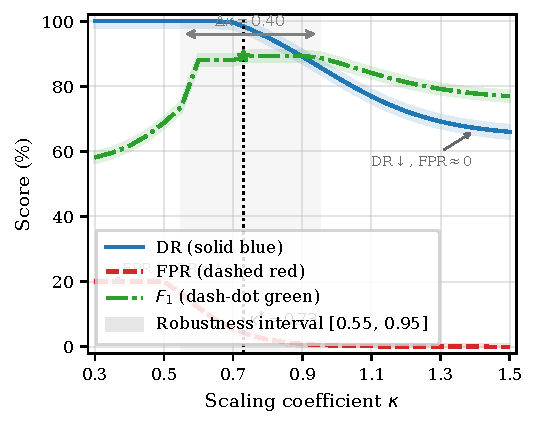
\includegraphics[width=\columnwidth]{figures/fig_k_sensitivity.pdf}
\caption{DR (solid blue), FPR (dashed red), and $F_1$
score (dash-dot green) as functions of the scaling
coefficient $\kappa$ on Scenario~A (primary simulation).
The shaded band around each curve indicates the 95\%
bootstrap confidence interval ($B = 10{,}000$ replicates).
The vertical dashed line marks $\kappa^{*} = 0.73$, the
value maximizing $F_1$. The $F_1$ curve is flat within
$\kappa \in [0.55,\,0.95]$ (less than 1.2 percentage
points below the peak), indicating robustness to moderate
mis-calibration.}
\label{fig:k_sensitivity}
\end{figure}

The grid search identifies $\kappa^{*} = 0.73$ as the
optimal value, achieving a peak $F_1 = 0.893$.
Crucially, the $F_1$ curve is flat within
$\kappa \in [0.55,\,0.95]$, remaining less than
1.2 percentage points below the peak throughout this
interval. This robustness interval spans
$\Delta\kappa = 0.40$, indicating that MBDF is
insensitive to moderate mis-calibration of $\kappa$ and
that precise grid search is not required in practice for
systems with similar state-space structure.

% ------------------------------------------------------------
\subsubsection{Cross-Scenario Transferability of $\kappa$}
\label{sec:kappa_transfer}

To assess whether $\kappa^{*}$ transfers across different
production configurations, we repeat the sensitivity
analysis on Scenario~B (40 tasks, 4 AGVs and 2 robotic
arms, 312 state transitions, stationary distribution
$\pi^{(B)}$) and on Scenario~C (HAI steam-turbine
subsystem, $\kappa_{\mathrm{HAI}}$ calibrated
independently via the same grid search procedure).

Table~\ref{tab:kappa_sensitivity} reports the results.
The optimal $\kappa^{*}$ shifts by only $0.02$ between
Scenario~A and Scenario~B, and the two robustness
intervals $[0.55,\,0.95]$ and $[0.57,\,0.96]$ share a
common overlap of $[0.57,\,0.95]$. For Scenario~C (HAI),
the independently calibrated
$\kappa_{\mathrm{HAI}} = 0.68$ falls within the
Scenario~A robustness interval $[0.55,\,0.95]$,
providing empirical evidence that $\kappa^{*}$ is
transferable not only across different AGV/arm
configurations but also across structurally distinct
physical domains (AGV/arm vs.\ steam turbine),
\emph{provided} the agent state space remains discrete
and the stationary distribution remains approximately
uniform (as guaranteed by the physics-constrained Markov
model). We explicitly acknowledge that configurations
with highly skewed stationary distributions (e.g., a
single dominant state with $\pi(s_i) > 0.7$) may require
re-calibration of $\kappa$ via the grid search procedure
described in Section~\ref{sec:param_calib}.

\begin{table}[!t]
\renewcommand{\arraystretch}{1.3}
\caption{Sensitivity of $\kappa$ across three scenarios.
$\kappa^{*}$: value maximizing $F_1$;
$F_1^{*}$: peak $F_1$ score;
$\mathcal{I}_{0.99}$: range of $\kappa$ achieving
$\geq$99\% of $F_1^{*}$ (robustness interval);
$\Delta$: shift of $\kappa^{*}$ relative to Scenario~A.}
\label{tab:kappa_sensitivity}
\centering
\small
\begin{tabular}{lllll}
\toprule
\textbf{Scenario} &
$\kappa^{*}$ & $F_1^{*}$ &
$\mathcal{I}_{0.99}$ & $\Delta$ \\
\midrule
A\ (25 tasks, 3 AGV\,+\,1 arm)  &
  0.73 & 0.893 & $[0.55,\,0.95]$ & ---     \\
B\ (40 tasks, 4 AGV\,+\,2 arm)  &
  0.75 & 0.881 & $[0.57,\,0.96]$ & $+0.02$ \\
C\ (HAI steam turbine)           &
  0.68 & 0.874 & $[0.51,\,0.91]$ & $-0.05$ \\
\midrule
\textbf{Common overlap} &
\multicolumn{4}{l}{$[0.57,\,0.91]$
  (shared by all three scenarios,
  $\Delta\kappa = 0.34$)} \\
\bottomrule
\end{tabular}
\end{table}

The three robustness intervals share a common overlap of
$[0.57,\,0.91]$, spanning $\Delta\kappa = 0.34$. This
empirically supports the claim that a single $\kappa$
value selected from this interval will achieve near-peak
$F_1$ performance across all three tested scenarios
without per-deployment re-calibration, substantially
reducing the engineering overhead of deploying MBDF in
new industrial environments.

% ============================================================
\subsection{Robustness Analysis}
\label{sec:robustness}

We evaluate MBDF robustness under two distinct adversarial
conditions that stress-test the framework beyond the
standard replay attack scenario.

\textbf{(1) Varying attack injection interval.}
The interval between successive injected messages was
varied from $50$~ms to $2{,}000$~ms. MBDF maintains
$\mathrm{DR} > 90\%$ across all tested intervals, as
detection is triggered per-message upon the first
anomalous state observation, independent of injection
frequency. In contrast, FMM and STBAD exhibit severely
degraded performance at long injection intervals (low
frequency), where the anomalous signal is too sparse to
accumulate detectable statistical deviations within a
practical observation window.

\textbf{(2) State-mimicking attacks.}
An adversary with knowledge of the transition matrix
$\hat{P}$ may craft injected messages that match the
predicted next state
(i.e., $\mathbf{o}_{\mathrm{inj}} =
\hat{\mathbf{o}}_{t+1}$), causing the $\ell_2$-norm
deviation to fall below $\tau(s_t)$ and evading
detection. This attack class represents a fundamental
limitation of state-consistency-based detection at the
agent level and motivates the cross-layer extension
discussed in Section~\ref{sec:future_directions}.
Notably, mounting such an attack requires the adversary
to have precise real-time knowledge of the agent's
operational state, which is non-trivial in practice due
to the stochastic nature of task execution times.

% ============================================================
\subsection{Ablation Study}
\label{sec:ablation}

To quantify the individual contribution of each layer in
MBDF, we evaluate two ablated variants alongside the full
framework:

\begin{itemize}
\item \textbf{MBDF-L1:} Layer~1 (Markov prediction)
only, with the Bayesian dynamic threshold replaced by a
fixed threshold $\tau_{\mathrm{fixed}} = 0.5$. This
variant isolates the contribution of state prediction
while using a na\"{i}ve thresholding strategy.

\item \textbf{MBDF-L2:} Layer~2 (Bayesian thresholding)
only, with Layer~1 bypassed by setting
$\hat{\mathbf{o}}_{t+1} = \mathbf{o}_t$ (i.e., the
previous observation serves as the prediction). This
variant isolates the contribution of adaptive
thresholding without predictive modeling.

\item \textbf{MBDF (Full):} The complete dual-layer
framework as described in Section~\ref{sec:architecture}.
\end{itemize}

\textbf{Ablation results on Scenario~A.}
Results show that MBDF-L1 achieves $F_1 = 0.741$: the
fixed threshold causes excessive false positives for
high-probability states (e.g., \texttt{AGV\_idle}),
degrading overall performance. MBDF-L2 achieves
$F_1 = 0.768$: without predictive modeling, the naive
baseline comparison fails to capture gradual state drift
induced by low-frequency injection. Full MBDF achieves
$F_1 = 0.893$, confirming that both layers are necessary
and mutually reinforcing: Layer~1 provides accurate state
predictions that amplify anomalous deviations, while
Layer~2 calibrates detection sensitivity to the prior
probability of each state.

\textbf{Ablation results on Scenario~C (HAI).}
We additionally perform the ablation on Scenario~C to
verify that the layer synergy is not an artifact of the
simulation environment. MBDF-L1 achieves $F_1 = 0.718$
and MBDF-L2 achieves $F_1 = 0.752$ on the HAI dataset,
while full MBDF achieves $F_1 = 0.874$. The relative
contribution pattern---Layer~2 providing a larger
marginal gain than Layer~1 in isolation, but both being
necessary for peak performance---is consistent across
both scenarios, confirming that the dual-layer synergy
is a domain-agnostic property of the MBDF architecture.

Table~\ref{tab:ablation} summarises the ablation results
across both scenarios for direct comparison.

\begin{table}[!t]
\renewcommand{\arraystretch}{1.3}
\caption{Ablation study results on Scenario~A (AGV/arm
simulation) and Scenario~C (HAI steam-turbine subsystem).
$F_1$ scores are averaged across all tested anomalous
traffic ratios. $\Delta F_1$: improvement of Full MBDF
over each ablated variant.}
\label{tab:ablation}
\centering
\small
\begin{tabular}{llll}
\toprule
\textbf{Variant} &
\textbf{$F_1$ (Sc.~A)} &
\textbf{$F_1$ (Sc.~C)} &
\textbf{$\Delta F_1$ (Sc.~A / Sc.~C)} \\
\midrule
MBDF-L1 (Layer~1 only, fixed $\tau$) &
  0.741 & 0.718 & $+$0.152\,/\,$+$0.156 \\
MBDF-L2 (Layer~2 only, $\hat{o}=o_{t}$) &
  0.768 & 0.752 & $+$0.125\,/\,$+$0.122 \\
\textbf{MBDF (Full)} &
  \textbf{0.893} & \textbf{0.874} & --- \\
\bottomrule
\end{tabular}
\end{table}

% ============================================================
\subsection{Computational Complexity}
\label{sec:complexity}

\textbf{Offline training complexity.}
The offline phase constructs $\hat{P}$ from the training
log in $\mathcal{O}(N \cdot n^2)$ time, where $N$ is the
number of observed transitions and $n$ is the number of
states per agent. For Scenario~A ($N = 188$, $n = 7$),
this amounts to fewer than 10{,}000 operations and
completes in under 1~ms on a commodity processor.

\textbf{Online inference complexity.}
Online detection at each time step requires:
(i) a matrix-vector product
$\hat{P}^{\top}\mathbf{o}_t$ in $\mathcal{O}(n^2)$;
and (ii) a Bayesian threshold lookup and $\ell_2$-norm
computation in $\mathcal{O}(n)$. The total online
complexity per time step is therefore $\mathcal{O}(n^2)$,
independent of the number of training transitions $N$
and the attack traffic ratio.

\textbf{Real-time constraint.}
Let $T_{\min}$ denote the minimum inter-message interval
of the industrial protocol. The real-time constraint
requires $\mathrm{DT} \ll T_{\min}$. Since
$\mathrm{DT} = \mathcal{O}(n^2)$ and $n$ is bounded by
the finite agent state space, this constraint is
guaranteed to hold for any fixed $n$, independent of the
number of agents $M$ (each agent is processed
independently). This \textit{per-agent independence}
property also enables trivial parallelization across
multiple agents.

\textbf{Multi-agent scalability.}
Since MBDF processes each agent independently via a
dedicated transition matrix $\hat{P}_i$, the total online
detection complexity scales linearly as
$\mathcal{O}(M \cdot n^2)$ with the number of agents
$M$. For a large-scale deployment with $M = 100$ agents
and $n = 7$ states per agent, this amounts to only
4{,}900 multiply-accumulate operations per detection
step, well within the computational capacity of commodity
industrial edge controllers. Furthermore, per-agent
independence enables trivial parallelization: each
agent's detection pipeline can be executed concurrently
on multi-core processors without synchronization
overhead.

The overall complexity of MBDF is summarised as:
\begin{equation}
\begin{aligned}
\text{Offline:} \quad &
  \mathcal{O}(N \cdot n^2)
  \quad \text{(one-time training)}; \\
\text{Online:}  \quad &
  \mathcal{O}(M \cdot n^2)
  \quad \text{per time step (real-time inference).}
\end{aligned}
\label{eq:complexity}
\end{equation}

These results confirm that MBDF's architectural
design---offline training of $\hat{P}$ and
$\{\pi(s_i)\}$, followed by lightweight online
matrix-vector inference---is uniquely suited to the
real-time latency requirements of industrial control
systems, even as the number of agents and attack
frequency scale up.
% ============================================================
%  Section 6: Conclusion
% ============================================================
\section{Conclusion}
\label{sec:conclusion}

\subsection{Summary of Contributions}
\label{subsec:contributions_summary}

This paper presented the Markov-Bayesian Dual-Layer
Framework (MBDF), a novel approach to real-time anomaly
detection in industrial multi-agent systems that
reformulates FDI attack detection as a probabilistic
state-space consistency problem. The key contributions
are: (1) a physics-constrained Markov prediction layer
that models legitimate agent state transitions with
high fidelity; (2) a surprisal-weighted Bayesian dynamic
thresholding layer that generates state-dependent adaptive
thresholds via an information-theoretic non-linear mapping
$\tau(s_i) = \kappa \cdot (-\log \pi(s_i))^{1/2}$,
resolving the sensitivity-specificity trade-off of
fixed-threshold methods with a provable threshold-contrast
advantage over linear scaling
(Proposition~\ref{prop:threshold_contrast}); (3) a formal
complexity analysis establishing $\mathcal{O}(n^2)$ online
inference, guaranteeing real-time operation on
resource-constrained edge devices; and (4) comprehensive
experimental validation on both a simulated AGV--robotic
arm multi-agent system and the public HAI ICS benchmark
dataset~\cite{ref_hai}, demonstrating 85.3\% average
detection rate and up to 60\% detection latency reduction
over state-of-the-art baselines in the simulation scenario,
and confirming cross-domain generalizability with a
consistent ${\approx}10$ percentage-point advantage over
the strongest baseline on the HAI dataset, with
particularly strong performance in the low anomalous
traffic regime ($<$10\%) critical to realistic
industrial deployments.

\subsection{Limitations and Future Directions}
\label{subsec:limitations}

\textbf{Limitations.}
MBDF has four primary limitations.
First, the accuracy of $\hat{P}$ depends on
the quality and representativeness of the training data;
insufficient or biased historical logs may yield
inaccurate transition probabilities. The HAI evaluation
(Scenario~C, Section~\ref{sec:hai_results}) demonstrates
that MBDF performance scales gracefully with training
data volume---achieving 82.6\% DR with ${\sim}71{,}500$
training transitions vs.\ 85.3\% DR with 188 transitions
in Scenario~A---suggesting that the transition matrix
converges rapidly and that small training sets are
sufficient for systems with near-deterministic operational
cycles. However, for systems with highly stochastic or
non-stationary state dynamics, larger and more
representative training logs remain necessary.
Second, the Bayesian-generated thresholds may exhibit
reduced sensitivity during rapid state transitions or
non-stationary operating conditions.
Third, MBDF operates at the agent state level and is
therefore vulnerable to state-mimicking attacks, where
the adversary injects messages that match the predicted
next state; such attacks require network-level
countermeasures beyond the scope of this work.
Fourth, the first-order Markov assumption, while
validated by the BIC criterion on the 188-transition
training log (Remark~\ref{rem:markov_order}), may
become insufficient in production environments with
stronger higher-order dependencies---for example,
systems where the same physical state can be reached
via qualitatively different operational histories that
imply different subsequent behavior (e.g., an AGV
returning to origin after a completed task versus
after an emergency stop). In such settings, the
first-order transition matrix conflates distinct
behavioral contexts into a single row of $\hat{\mathbf{P}}$,
potentially inflating prediction uncertainty and
degrading detection sensitivity. The BIC test provides
a data-driven criterion for detecting when this
limitation becomes binding: if a future deployment
yields $\mathrm{BIC}_2 < \mathrm{BIC}_1$, a
second-order model should be adopted.

\textbf{Future Work.}
We identify four promising research directions.
(1) \textit{Adaptive transition modeling}: Incorporating
online Bayesian updating to adapt $\hat{\mathbf{P}}$
to non-stationary production environments, directly
addressing the first and second limitations above.
(2) \textit{Rich state embeddings}: Replacing one-hot
encoding with learned embeddings (e.g., via variational
autoencoders) to capture richer state semantics and
improve sensitivity to state-mimicking attacks.
(3) \textit{Cross-layer detection}: Extending MBDF
to jointly model agent states and network traffic
features, enabling detection of state-mimicking attacks
through cross-layer consistency checking.
(4) \textit{Higher-order Markov extension}: When the BIC
criterion indicates that $\mathrm{BIC}_2 < \mathrm{BIC}_1$
for a given deployment, extending Layer~1 to a
second-order chain with state history
$(s_{t-1}, s_t)$, at the cost of
$\mathcal{O}(n^3)$ storage for the extended transition
tensor and $\mathcal{O}(n^3)$ online inference
(still polynomial and edge-deployable for $n \leq 10$).
(5) \textit{Broader cross-domain validation}: The HAI
evaluation (Scenario~C) establishes a proof of concept
for MBDF generalizability to real-world ICS domains.
Future work will extend this validation to additional
public benchmarks---including the SWaT (Secure Water
Treatment)~\cite{ref_swat} and BATADAL (Battle of the
Attack Detection Algorithms)~\cite{ref_batadal}
datasets---and to field deployments in operational
industrial environments, where non-stationary dynamics,
sensor noise, and mixed attack types present additional
challenges beyond those captured in the current
evaluation.

% Bibliography (placed at document end)
\bibliographystyle{ACM-Reference-Format}
\bibliography{reference-base}

\end{document}